\documentclass[conference]{IEEEtran}
\IEEEoverridecommandlockouts
% The preceding line is only needed to identify funding in the first footnote. If that is unneeded, please comment it out.
\usepackage{cite}
\usepackage{amsmath,amssymb,amsfonts}
\usepackage{graphicx}
\usepackage{textcomp}
\usepackage{xcolor}
\usepackage{subfig}
\usepackage{algorithm}
\usepackage{algpseudocode}
\usepackage{diagbox}
\usepackage{footnote}
\usepackage{bbding} %\Checkmark \XSolid
% to be able to draw some self-contained figs
\usepackage{tikz}
% inlined bib file
\usepackage{filecontents}

\newcommand{\pushcode}[1][1]{\hskip\dimexpr#1\algorithmicindent\relax}

\def\BibTeX{{\rm B\kern-.05em{\sc i\kern-.025em b}\kern-.08em
    T\kern-.1667em\lower.7ex\hbox{E}\kern-.125emX}}
\begin{document}

\title{Exploit Lock Violation for Fault-tolerant Distributed Database System}


\author{\IEEEauthorblockN{Hua Guo}
\IEEEauthorblockA{\textit{School of Information} \\
\textit{Renmin University of China}\\
Beijing, China \\
guohua2016@ruc.edu.cn}
\and
\IEEEauthorblockN{Xuan Zhou}
\IEEEauthorblockA{\textit{School of Data Science And Engineering} \\
\textit{East China Normal University}\\
Shanghai, China \\
xzhou@dase.ecnu.edu.cn}
}

\maketitle

\begin{abstract}
Modern distributed database systems scale horizontally by sharding its data on a large number of nodes.
To achieve fault tolerance, most of such systems build their transactional layers on a replication layer,
which employs a consensus protocol to ensure data consistency.
Synchronization among replicated state machines thus becomes a major overhead of transaction processing.
Without a careful design, synchronization could amplify transactions' lock duration and impair the system's scalability.
Speculative techniques, such as Controlled Lock Violation (CLV) and Early Lock Release (ELR), prove to be effective in shortening lock duration and boosting performance of transaction processing.
An intuitive idea is to use these techniques to optimize geo-replicated distributed databases.
In this paper, we show that direct application of speculation is often unhelpful in a distributed environment.
Instead, we introduce Distributed Lock Violation (DLV), a speculative technique for geo-replicated distributed databases.
DLV minimize the cost of to conduct lock violation, so that it can achieve good performance without incurring severe side effects.
\end{abstract}

\begin{IEEEkeywords}
Database System, Distributed Transaction, Locking, High Availability
\end{IEEEkeywords}

\section{Introduction}

Modern distributed database system scale out by partitioning data across multiple nodes, so that it can run transactions on multiple servers in parallel to increase throughput.
When a transaction needs to access multiple partitions, it has to employ a coordination protocol to ensure atomicity.
It is commonly known that such distributed transactions can lead to significant performance degradation.
This is mainly due to the following reasons\cite{Calvin:conf/sigmod/ThomsonDWRSA12}:

1. Coordinated commit requires a chatty protocol (e.g., Two-Phase Commit), which introduces tremendous network overheads;

2. Message transmission overlaps with the critical path of transaction commit, which worsens the contention among transactions.

These issues can be more serious for geo-replicated databases, which face increased network overheads.
%Transactional layer uses a specific concurrency control(CC) scheme to enforce a serializable schedule and a distributed commit protocol if transaction access multiple shards.
%Optimistic CC scales well when there is little contention but suffers high abort rate when it dealing with a workload of high degrees of contention.
%Pessimistic CC has a lower abort rate, but it endures overheads of blocking.
%In fact, CC matters little on performance if no conflicts and no most CC schemes failed to handle high contention\cite{PerformanceOfCC:conf/vldb/CareyS84}\cite{EvaluationOfCC:journals/pvldb/HardingAPS17}.
The replication layer of a geo-replicated database often uses a Paxos-like consensus protocol to ensure consistency among replicas.
This introduces a significant amount of message transmission, which further increase the duration of transactions.
To facilitate replication, we usually split data into small chunks and replicate each chunk independently.
As a result, cross-chunk transactions (rather than cross-partition transactions) all become distributed transactions.
This makes distributed transaction even more inevitable.

\begin{figure}[htbp]
  \centerline{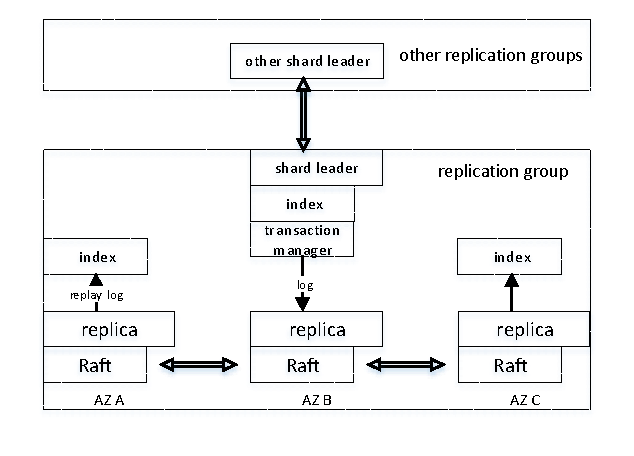
\includegraphics[scale=0.8]{figure/architecture.pdf}}
  \caption{Typical architecture of geo-replicated distributed DBMS}
  \label{fig:architecture}
\end{figure}

Fig~\ref{fig:architecture} presents the typical architecture of geo-replicated distributed databases.
The database partitions its data into a number chunks.
For each chunk, the replication layer replicates its data to several Availability Zones (AZ) \cite{Aurora:conf/sigmod/VerbitskiGSCGBM18}.
Among the available zones, the replication layer employ a consensus protocol to shield data consistency.

As previous work has discussed \cite{Calvin:conf/sigmod/ThomsonDWRSA12}\cite{Tapir:conf/sosp/ZhangSSKP15}\cite{Janus:conf/osdi/MuNLL16},
this architecture has to rely on a chatty protocol (which integrates the commit protocol and the consensus protocol) to ensure the correctness of transactions.
It may fail to scale when confronted with highly contended workload.
Nevertheless, this architecture supports a wide range of transaction processing methods.
Most industrial data systems choose this two-layer architecture, including Google Spanner \cite{Spanner:conf/osdi/CorbettDEFFFGGHHHKKLLMMNQRRSSTWW12}\cite{Spanner:conf/sigmod/BaconBBCDFFGJKL17},
NuoDB \cite{NuoDB}, CockroachDB \cite{CockroachDB}, TiDB \cite{TiDB}, etc.

\begin{figure}[htbp]
  \centerline{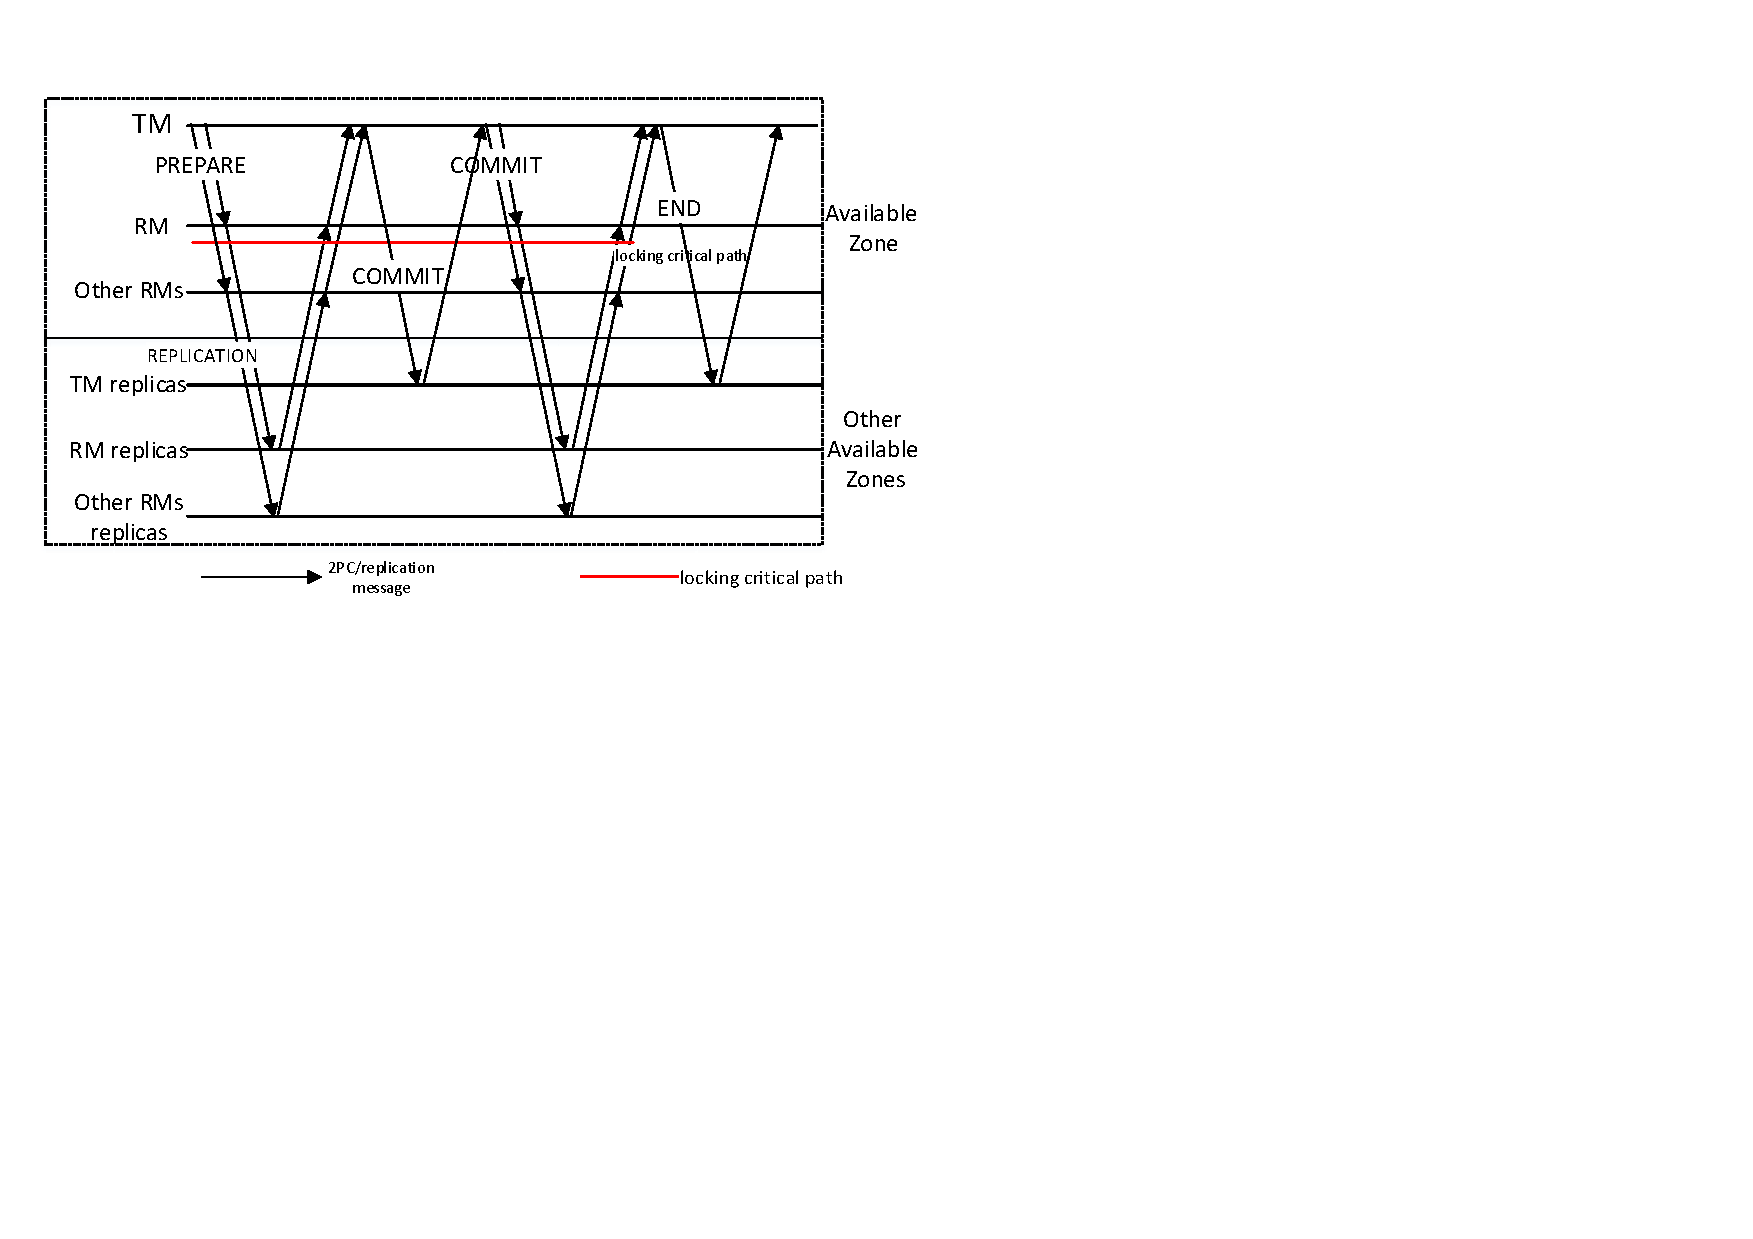
\includegraphics[scale=0.62]{figure/message_flow.pdf}}
  \caption{The message flow and lock holding critical path when the DBMS uses S2PL for concurrency control and 2PC as the commit protocol.
The dash arrow lines represents the messages introduced by Distributed Lock Violation (DLV). The red lines represent the critical paths of S2PL.
The green dash lines represent the critical paths of DLV.}
  \label{fig:two_layers_architecture}
\end{figure}

Looking more closely, the main issue is that the commit and consensus protocols enlarge the timespan of the critical paths in transaction processing.
This significantly amplifies the overhead of contention.
%We focus on distributed DBMS which uses locking scheme and coordination protocol on a replicated layer, especially who running transaction processing on geo-replicated layer.
Fig \ref{fig:two_layers_architecture} shows the message flow of a distributed transaction in such an architecture. We assume that
it uses S2PL for concurrency control and 2PC as the commit protocol, and the replication layer is deployed over a WAN.
When a transaction requests to commit, the \emph{TM (transaction manager)} issues a `prepare' message to each \emph{RM (resource manager)}.
Then, each \emph{RM} replicates its vote (`prepare commit' or `prepare abort') to the corresponding replicas through a consensus protocol, before it
sends its vote to \emph{TM}.
After the \emph{TM} collects all the votes of the \emph{RMs},
it broadcasts the final decision (`commit' or `abort') to all the \emph{RMs}
\footnote{Depending on variants of implementations, the TM can choose to persist its decision on its log or not.}
.
Once a \emph{RM} receives the final decision from the \emph{TM}, it replicates the decision to the corresponding replicas.
After the consensus of commit or abort is reached, the \emph{RM}
can release the locks that it had retained over the accessed data.

We depict lock duration by red lines in Fig~\ref{fig:two_layers_architecture}.
As we can see, the lock duration span multiple message round trips, including those over the WAN.
This will severely impair the concurrency of transaction processing in face of a high degree of contention.

Speculative techniques, such as Early Lock Release (ELR) \cite{EfficientLocking:conf/vldb/KimuraGK12} and Controlled Lock Violation (CLV)
\cite{CLV:conf/sigmod/GraefeLKTV13}, prove to be effective in optimizing centralized transaction processing.
These techniques can be extended to a distributed environment.
%The two-layer architecture shares the same bottleneck with single node DBMS on forcing transaction log and faces even worse conditions.
%Fig \ref{fig:log_write_latency} shows the log write latency of different environment(TODO... experiments setting).

\begin{figure}[htbp]
  \centerline{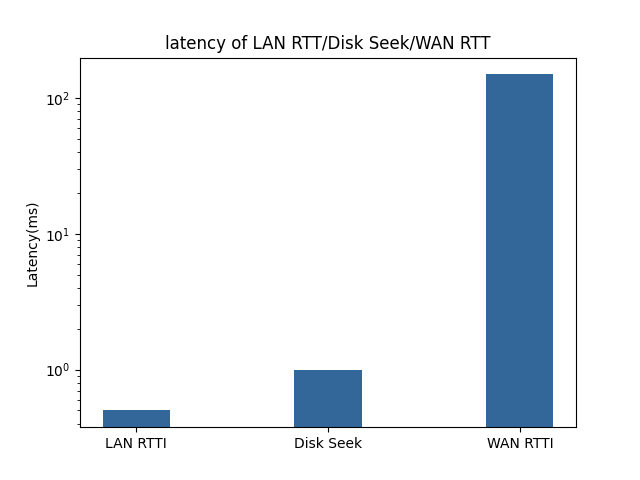
\includegraphics[scale=0.4]{figure/log_write_latency.png}}
  \caption{approximate latency comparison\cite{Latency}}
  \label{fig:log_write_latency}
\end{figure}

Speculative techniques improve concurrency by excluding logging from lock duration,
Transactions on geo-replicated distributed databases require much more time to ship and persist logs.
Fig \ref{fig:log_write_latency} shows the WAN RTT , LAN RTT and disk seek approximate time costs comparison.
This provides more opportunities for exploiting speculation.
However, application of speculation in a distributed environment is complex.
A number of design choices need to be considered.
For instance, when working with 2PC, we need to decide to violate (or release) lock at which phase.
As previous work showed \cite{CLV:conf/sigmod/GraefeLKTV13}, lock violation at the first phase may enable a higher degree of concurrency.
However, dependency tracing and cascade abort may incur excessive overheads.
On the contrary, lock violation at the second phase costs less in dependency tracing and cascade abort, while it has to sacrifice a certain amount of concurrency.
%Transaction models, interactive or one-shot transactions, may have different message flow, how different transaction types could benefit from these techniques?
On the other hand, not all transactions can benefit from CLV or ELR, e.g., workload with little conflict.
It unnecessary and even harmful to apply speculation to all cases.

In this paper, we propose a technique called Distributed Lock Violation (DLV) to enhance the performance of geo-replicated distributed DBMS.
DLV decides the best time to perform lock violation by looking at runtime statistic information.
It introduces much less penalty compared to previous implementation \cite{CLV:conf/sigmod/GraefeLKTV13}.

The remainder of this paper is organized as follows.
Section \ref{sec:relate_work} reviews related work.
Section \ref{sec:non_strict} shows that a strict schedule is not necessary and hurt the performance of distributed DBMS.
Section \ref{sec:implement} introduces DLV.
Section \ref{sec:experiments} evaluates DLV and compare it against previous work.
Section \ref{sec:conclution} concludes this paper.


\section{Relate Work}
\label{sec:relate_work}
%This section introduces the related work of this paper.

\subsection{Transaction Processing on Replicated Databases}
%Recently, there are many scalable DBMS arisen in both academia and industry.
%Most of the systems in this category supports distributed query processing and
%replicate data across several data center geo-located in different areas for fault tolerance.

Most replicated databases rely on state-machine replication(SMR) to realize high availability.
SMR often uses a consensus protocol to synchronize different replicas.
Synchronization introduces significant amount of network traffic and becomes a major overhead of replicated database systems.
Paxos \cite{Paxos:journals/tocs/Lamport98}\cite{PaxosSimple:conf/opodis/Lamport02} is the most well known consensus protocol.
To reach a consensus on a single data update in Paxos, it costs two message round trips, one for choosing a proposal and another for proposing the entry.
Multidecree Paxos\cite{Multidecree:journals/csur/RenesseA15} elects a leader as the only proposer to eliminate the first message round trip.
Raft\cite{Raft:conf/usenix/OngaroO14} is a similar consensus protocol to Paxos. As it is more understandable, it is widely used in modern database systems.
In Raft, it costs at least one message round trip to reach a consensus.
Google Spanner \cite{Spanner:conf/osdi/CorbettDEFFFGGHHHKKLLMMNQRRSSTWW12}\cite{Spanner:conf/sigmod/BaconBBCDFFGJKL17},
NuoDB \cite{NuoDB}, CockroachDB \cite{CockroachDB} and TiDB \cite{TiDB} are all geo-replicated DBMSes built upon Paxos or Raft.
They all face heavy costs incurred by data synchronization.

To minimize the cost of synchronization, a number of techniques have also been proposed.
VoltDB \cite{VoltDB} and Calvin \cite{Calvin:conf/sigmod/ThomsonDWRSA12} employ a deterministic transaction model
to reduce the coordination cost of distributed transactions.
Deterministic scheduling enables active replication, which allows transactions to kickoff synchronization at the earliest possible time.
Tapir \cite{Tapir:conf/sosp/ZhangSSKP15} relaxes the consistency requirements of the replication layer, so that it can reduce the message round trips to reach consensus.
Janus \cite{Janus:conf/osdi/MuNLL16} aims to minimize wide-area message round trips
by consolidating the concurrency control mechanism and the consensus protocol.
It uses deterministic serializable graph tracing to ensure atomicity of transactions.
In a nutshell, Tapir and Janus both co-designed the transaction and replication layers of distributed databases, so that they only need to incur one wide-area message round trip to commit a transaction.
VoltDB, Calvin, Tapir and Janus all impose strict constraints on the implementation of the transaction layer, making them incompatible with existing systems, such as Spanner and CockroachDB.
In contrast, this work focuses on the optimization opportunities in the general implementation of geo-replicated databases (as depicted in Fig~\ref{fig:architecture}).

\subsection{Optimization on Locking based Concurrency Control}
%DBMS use concurrency control(CC) to calculate a serializable schedule for concurrent transactions.
Two-phase locking (2PL) is the most widely used concurrency control mechanism.
As a pessimistic method, 2PL assumes a high likelihood of transaction confliction.
It uses locks to enforce the order of conflicting transactions.
Strict 2PL (S2PL) is a brute force implementation of 2PL. 
It requires a transaction to preserve all its lock until it ends.
As S2PL can easily guarantee transactions' recoverability, many databases choose to use it.
When extending S2PL to distributed databases, the lock holding time will be substantially enlarged, 
as the commit critical path will involve a number of message round trips.

All S2PL implementations adopt a certain approach to resolve deadlocks.
In the \emph{no-wait}
\cite{EvaluationOfCC:journals/pvldb/HardingAPS17}
approach, a transaction immediately aborts if it fails to place a lock.
Previous works showed that this is a scalable approach in a distributed environment \cite{EvaluationCC1000Cores:journals/pvldb/YuBPDS14}\cite{EvaluationOfCC:journals/pvldb/HardingAPS17},
as it eliminates blocking completely.
However, it works poorly when dealing with workload of high contention.
Another approach is \emph{wait-die} \cite{LockNoWait:journals/csur/BernsteinG81}. 
It avoids some false-positive aborts encountered by \emph{no-wait} by utilizing timestamps.
The \emph{Deadlock detection} approach \cite{LockCC:conf/ds/GrayLPT76} detects deadlock by explicitly tracing wait-for relationship among transactions.
Many centralized database systems \cite{MySQL}\cite{PostgreSQL} adopt this approach, as can deal with contention better.
However, deadlock detection in a distributed environment is highly costly, making it the least favorable approach in our case.

%\subsection{Exploit Speculation and Lock Violation}
To optimize the performance of locking based concurrency control, speculation can be used.
%Similar approaches have been introduced by many previous works.
Early lock release (ELR)
\cite{ELR:dewitt_implementation_1984}\cite{PS2PL:conf/icdt/Soisalon-SoininenY95}
\cite{Aether:journals/pvldb/JohnsonPSAA10}
\cite{EfficientLocking:conf/vldb/KimuraGK12}
\cite{Actor-Oriented-DB:conf/icde/Bernstein18}
is a typical speculative technique.
ELR allows a transaction to release its locks before its commit log is flushed to disk.
It was first proposed by DeWitt et al.\cite{ELR:dewitt_implementation_1984}.
Soisalon-Soininen et al.\cite{PS2PL:conf/icdt/Soisalon-SoininenY95} analyzed its correctness in various settings.
Many other works applied and evaluated ELR in different types of systems \cite{Aether:journals/pvldb/JohnsonPSAA10}\cite{EfficientLocking:conf/vldb/KimuraGK12}\cite{EfficientLocking:conf/vldb/KimuraGK12}\cite{Aether:journals/pvldb/JohnsonPSAA10}.
However, previous works on ELR were limited to centralized database systems.
%Jones et al.\cite{LowOverheadCC:conf/sigmod/JonesAM10} use a restirct transaction model\cite{H-store:journals/pvldb/KallmanKNPRZJMSZHA08} implement sepculation.

Control lock violation (CLV) \cite{CLV:conf/sigmod/GraefeLKTV13} is a more general speculative technique than ELR.
It allows certain transactions to ignore certain locks, instead of releasing a lock completely.
CLV has been tested on distributed databases. The results show that it can optimize both phases of two-phase commit.
CLV needs to trace dependency among transactions.
In \cite{CLV:conf/sigmod/GraefeLKTV13}, the authors use a Register and Report (RARA) approach \cite{HeckatonMVCC:journals/pvldb/LarsonBDFPZ11} to implement the tracer.
RARA work well on a centralized database. In a distributed environment, dependency tracing becomes much more costly.
Cascade abort is another side effect of speculation. It can also leads to severe performance downgrade for distributed databases.


\section{Scheduling with Lock Violation}
\label{sec:non_strict}

In the following, we describe the basic idea of scheduling with lock violation.

\subsection{Preliminaries and Assumptions}
Our scenario is a geo-replicated distributed database, which shards its data by primary keys.
Each data chunk is replicated across a number of remotely located AZs.
Physiological logs are transmitted among the AZs to keep the data synchronized.
The physiological logs record the row-level write operations of each transaction.
A consensus protocol to used to prevent the synchronization from going wrong.
%Other replication protocols may also work.
We assume that there is a replica leader for each data chunk, which is responsible for coordinating the synchronization process.

We assume that two types of distributed transactions can be conducted on the system. They are known as one-shot and interactive transactions.
Fig \ref{fig:transaction_type} shows the message flow during the commit phase of the two types of transactions.
We can see that an interactive transaction costs more message round trips than a one-shot transaction,
as the $TM$ has to explicitly notify the $RM$s that they can prepare to commit.
%These two types of transaction model employ different message flow.
%Our lock violation technique must work with both types of transactions, which we will explain subsequently.

\begin{figure}[htbp]
    \centering
    \captionsetup[subfigure]{oneside,margin={0.3cm,0cm}}
    \subfloat[one-shot transaction, which does not need to explicitly ask the $RM$s to prepare]
        { 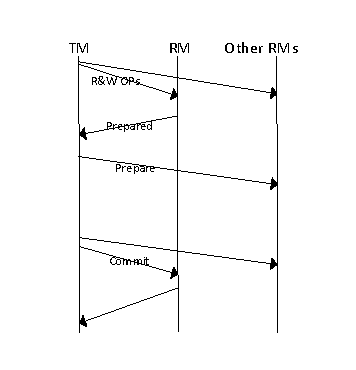
\includegraphics[scale=1] {figure/transaction_oneshot}  \label{fig:transaction_oneshot}  }
    \captionsetup[subfigure]{oneside,margin={0.3cm,0cm}}
    \subfloat[interactive transaction, which has to notify each $RM$ to prepare ]
        { 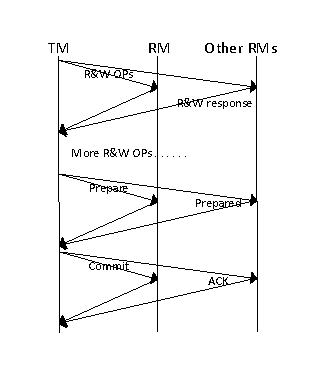
\includegraphics[scale=1]{figure/transaction_interactive} \label{fig:transaction_interactive}}

  \caption{Commit message flows for one-shot and interactive distributed transactions}
  \label{fig:transaction_type}
\end{figure}



\subsection{Concepts of Scheduling}
Before presenting the idea of lock violation, we first review the conceptual model of transaction processing. Most of the contents can be found in previous work, such as \cite{LockNoWait:journals/csur/BernsteinG81}.

\subsubsection{Transaction and History}
Suppose that a distributed database resides on ${n}$ nodes, represented by ${R = \{r_1, r_2, ... r_n\}}$.
A transaction ${T_i}$ can run on any ${m}$ of the ${n}$ nodes ($1 \le m \le n$), represented by  ${S = \{s_1, s_2, ... s_m\} \subseteq R}$,
The transaction ${T_i}$ is composed of a series of operations, %, represented by ${O = \{o_1, o_2, ... o_k\}}$.
%Each $o_i \in O$
where each can be a read or a write or other command operation including abort, commit, etc.
Let ${r_i[x]}$ denote that ${T_i}$ reads the record ${x}$. Let ${w_i[x]}$ denote that ${T_i}$ writes on the record ${x}$.
Let ${c_i}$, ${a_i}$, ${p^c_i}$, ${p^a_i}$ denote the commit, abort, prepare-to-commit and prepare-to-abort operations of ${T_i}$ respectively.
%We call ${T_i}$'s operations on the node ${s_u}$ ${T_i}$'s \emph{sub-transaction} on ${s_u}$.

A transaction history is a collection ${H = \{h_1, h_2, ..., h_n\}}$, in which
each ${h_u}$ is the local history of $H$ on the node ${s_u}$, which is a sequence of operations issued by different transactions.

%in which ${h_u (1 \le u \le n) = \Pi_u(H)}$ is the local history on site ${s_u}$.
%${\Pi_u(H)}$ is ${H}$'s projection on site ${s_u}$.
%For any projected history ${h_u(1 \le u \le m)}$, ${h_{u} }$ is a collection of  operations requests by many transactions.

\subsubsection{Deterministic and Non-deterministic Abort}
A number of reasons can cause a transaction to abort. In general, they can be categorized as:

1. User requested abort. These are aborts specified by the program logic (e.g., requiring a transaction to abort if it has accessed non-existent records).

2. Violation of isolation (e.g., serializability). These are aborts commanded by the database system.

3. Database node failure. For simplicity, we assume fail-stop failures only.

We call the first two types of abort \emph{deterministic abort} and the last one \emph{non-deterministic abort}.
In a database system, deterministic aborts occur much more frequently than non-deterministic abort.
Therefore, the prices we are willing to pay for the two kinds of abort are very different. 

\subsubsection{Dependencies among Transaction}

There are there kinds of data dependency among transactions, known as \emph{wr-dependency}, \emph{ww-dependency} and \emph{rw-dependency}.
In a local history ${h}$, if ${T_j}$ reads ${T_i}$'s write on ${x}$,
we call it a \emph{write-after-read(wr) dependency} and denote it by ${w_i[x] \rightarrow r_j[x]}$.
Analogically, if ${T_j}$ overwrites ${T_i}$'s write on ${x}$, it is called a \emph{write-after-write(ww) dependency} and denoted by ${w_i[x] \rightarrow w_j[x]}$.
If ${T_i}$ reads ${x}$ before ${T_j}$ writes on ${x}$, it is called a \emph{read-after-write(rw) dependency} and denoted by ${r_i[x] \rightarrow w_j[x]}$.

Based on data dependencies, we can define \emph{commit dependency}. ${T_j}$ has a \emph{commit dependency} on ${T_i}$, written as ${T_i \rightarrow T_j}$, if ${T_j}$ cannot commit prior to ${T_i}$.
In other words, ${T_i}$ aborts, ${T_j}$ has to abort too. ${T_j}$ has a \emph{commit dependency} on ${T_i}$, if and only if ${T_j}$ has a \emph{rw-dependency} on ${T_i}$.

%A transaction ${T_j}$ \emph{speculatively access} a record ${x}$, if there is another transaction ${T_i}$,
%${T_j}$ has a commit dependency on ${T_i}$ and  ${T_i}$ has not committed.
%We call such a commit dependency a \emph{danger dependency}, denote it as ${T_j \rightarrow_s T_i}$.

\subsubsection{Relaxation on Strictness}

Most traditional database systems adopt Strict Two-Phase Locking (S2PL) \cite{DBLP:conf/vldb/Raz92} to ensure the recoverability of transactions.
Strictness implies that a transaction cannot read a previous write by another transaction which has not committed yet.
%For a locking base concurrency control scheme, the lock will hold until the transaction end, namely strict two-phase locking(S2PL).

Strictness is not a necessary condition for a correct schedule.
Although it simplifies the implementation of a database system, it sacrifices the concurrency of transaction processing.
%\subsection{Strict Scheduler is Too ``Strict" for Correctness}
For instance, the schedule ${H_1}$ of Fig \ref{fig:strict_example} is serializable and strict. %there are 3 working nodes, ${s_1}$, ${s_2}$, ${s_3}$.
(The data dependencies include ${r_1[x] \rightarrow w_3[x]}$, ${w_1[x] \rightarrow r_2[y]}$, ${r_2[y] \rightarrow w_3[x]}$, which are not cyclical.)
In contrast, ${H_2}$ in Fig~\ref{fig:non_strict_example} is serializable but not strict.
In Fig~\ref{fig:non_strict_example}, there are three records ${x}$, ${y}$, ${z}$, residing on ${s_1}$, ${s_2}$, ${s_3}$ respectively.
${T_1}$ writes ${y}$ and ${x}$.
${T_2}$ reads ${T_1}$'s write on ${x}$ before ${T_1}$ commits.
Transaction ${T_3}$ overwrites ${T_2}$'s write before ${T_2}$ commits.
As we can see, by violating strictness, ${H_2}$  enables a higher degree of concurrency.

%The schedule ${H_2}$ can be represented as
%\begin{center}
%  ${H_2 = \{h_1, h_2, h_3\}}$,
%\end{center}
%in which,
%\begin{center}
%${h_1=w_1[x], w_3[x], p^c_1, c_1, p^c_3, c_3}$
%
%${h_2=w_1[y], r_2[y], p^c_1, c_1, p^c_2, c_2}$
%
%${h_3=r_2[z], w_3[z], p^c_2, c_2, p^c_3, c_3 }$.
%\end{center}


%Both of ${H_1}$ and ${H_2}$ are serializable equal with the serial schedule, ${T_1}$ ${T_2}$ ${T_3}$.
%Scheule ${H_1}$ and ${H_2}$ are correct.


\begin{figure}[htbp]
  \centerline{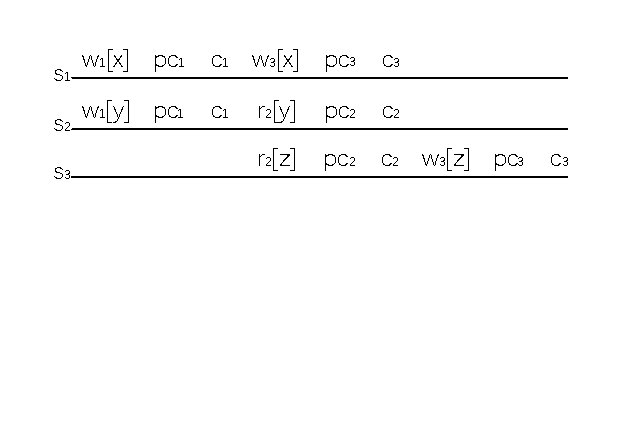
\includegraphics[scale=1]{figure/schedule_strict.pdf}}
  \caption{A strict and serializabile schedule ${H_1}$}
  \label{fig:strict_example}
\end{figure}

\begin{figure}[htbp]
  \centerline{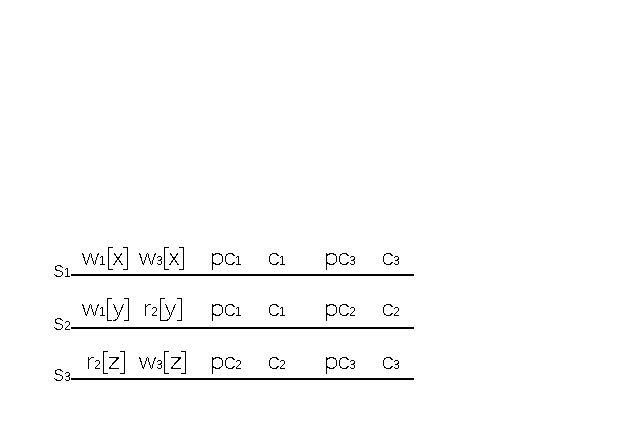
\includegraphics[scale=1]{figure/schedule_non_strict.pdf}}
  \caption{A non-strict but serializabile schedule ${H_2}$}
  \label{fig:non_strict_example}
\end{figure}

\begin{figure}[htbp]
  \centerline{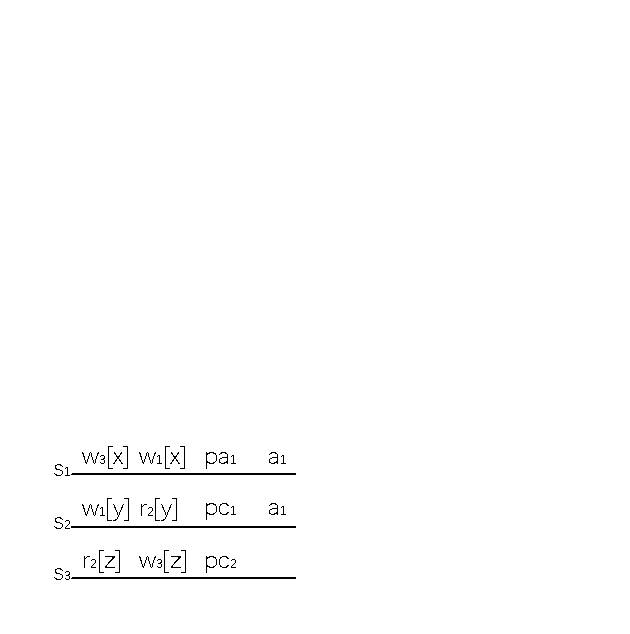
\includegraphics[scale=1]{figure/schedule_not_serializabile.pdf}}
  \caption{Schedule ${H_3}$, ${T_1}$ abort due to non-serializabile}
  \label{fig:schedule_abort_example}
\end{figure}

\begin{figure}[htbp]
  \centerline{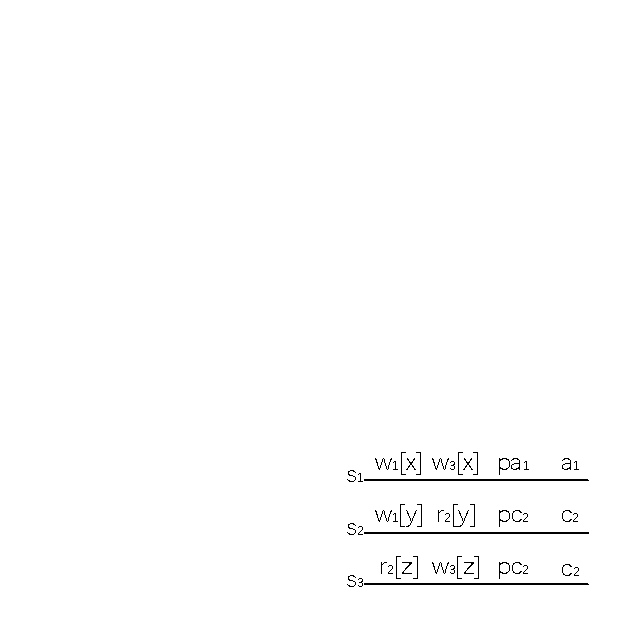
\includegraphics[scale=1]{figure/schedule_not_recoverable.pdf}}
  \caption{Schedule ${H_4}$, ${T_2}$ commit ahead ${T_1}$, non-recoverable anomaly}
  \label{fig:schedule_not_recoverable}
\end{figure}


%To realize such a schedule, ${T_1}$ must release its lock or mark it as violatable before it commits.

The drawback of strictness is amplified in a geo-replicated and distributed database.
The commit of a transaction in such a database usually involve a lot of work, including multiple rounds of communication across the WAN.
As strictness requires a transaction to hold locks until it finishes committing, this means a substantially lengthened lock holding time. 
This will hurt the performance of distributed transactions severely.
Our basic idea is to develop a serializable but non-strict scheduler to shorten the lock holding time.

Relaxation on strictness will, however, complicate the recovery mechanism.
In a traditional recovery mechanism, such as ARIES, the dependencies among transactions completely comply with the persisting order of their logs. %\cite{ELR:dewitt_implementation_1984}\cite{EfficientLocking:conf/vldb/KimuraGK12}.
This guarantees the recoverability of scheduling, which requires that a transaction cannot commit before the transactions it has commit dependencies on.
When strictness no longer holds, we need other tactics to enforce the commit order, which may incur additional overheads.

%When we extended the non-strict locking scheme to distributed transaction, transaction dependency maintaining is more complex.
%The serializable scheduler is a correct one if it can prevent abort.
%But when there are aborted transactions, it does not.
%To produce the correct log, the schedule must be both commit serializable and recoverable\cite{UnifyCR:journals/is/AlonsoVABASW94}.
%The scheduler need to maintain commit dependencies to guarantee serializability and recoverability when exploiting non-strictness.

\subsection{Lock Violation and Dependency Tracing}

Lock violation is a general technique to enable a non-strict scheduler.
Its basic idea is to allow a transaction to speculatively access data locked by other transactions.
If such speculative data accesses cause a problem, the system should be able to rectify it.

For lock violation to be correct, it should first preserve serializability.
Considering the non-strict schedule ${H_3}$ in Fig \ref{fig:schedule_abort_example},
it contains three data dependencies:

\begin{center}
${w_3[x] \rightarrow _s w_1[x]}$,
${w_1[y] \rightarrow _s r_2[y]}$
${r_2[z] \rightarrow _s w_3[z]}$
\end{center}

This leads to a circle ${T_1 \rightarrow T_2 \rightarrow T_3 \rightarrow T_1}$, which makes the schedule non-serializable.
${H_3}$ is not possible if we apply S2PL. It becomes possible when lock violation is permitted -- we allow
${T_2}$ to read from uncommitted ${T_1}$, and ${T_1}$ to overwrite uncommitted ${T_3}$.
Therefore, to preserve serializability, we need to prevent the data dependencies from forming a dependency cycle.
Many techniques can be adopted to achieve this, including the \emph{wait-die} strategy mentioned in the related work.

Secondly, a schedule generated by lock violation must be recoverable.
In the schedule ${H_4}$ in Fig~\ref{fig:schedule_not_recoverable}, due to lock violation,
${T_2}$ reads  ${T_1}$'s write and commits before ${T_1}$.
%There is a danger dependency, ${w_1[y] \rightarrow_s r_2[y]}$ and ${T_2}$ 's commit is ahead ${T_1}$'s commit.
In this case, if ${T_1}$ later on decides to abort, it is no longer possible to reverse ${T_2}$.
Therefore, ${H_4}$ is not a recoverable schedule.
%If ${T_1}$ abort, then ${T_2}$ will return an error ${y}$ value.
To ensure recoverability, we need to trace the commit dependencies (i.e., $wr$-dependencies) among transactions, and force the commit order to comply with the commit dependencies.
For instance, if we know that ${T_2}$ depends on ${T_1}$, we can hold ${T_2}$'s commit request until ${T_1}$ finishes.
If ${T_1}$ decides to abort, we abort ${T_2}$ too. This is known as cascade abort. 

In a geo-replicated distributed database, lock violation can potentially be allowed at two occasions in a transaction.
The first occasion is when the work of the transaction has been completed successfully and the transaction is ready to commit.
We call lock violation at this occasion \emph{late lock violation}. It is only intended to reduce the contention in the commit phases of transactions.
The second occasion is before the transaction is ready to commit. We call lock violation at this occasion \emph{early lock violation}. 
The early lock violation can also fall into two categories: 
that which violation when an ${RM}$ begins to decides its prepare decision, 
and violation when a transaction is even on-going in this ${RM}$. 

%Suppose ${H}$ is a schedule which is created by lock violation. We complement ${H}$  with the lock, unlock and lock violation operations,
%so it looks as follows:
%\begin{center}
%  ${H = l_i[x] o_i[x]... vl_j[x] o_j[x]...  l_i[y] o_i[y]... ul_i[x] ... }$
%\end{center}
%In ${H}$, ${x}$, ${y}$ are separate records.
%${T_i}$ first locks ${x}$ (i.e., $l_i[x]$).
%Then, ${T_j}$ violates  ${T_i}$'s lock on ${x}$ (i.e., $vl_j[x]$).
%Following that, ${T_i}$ locks ${y}$ and releases its lock on ${x}$ (i.e., $l_i[y]... ul_i[x]$).
%If a lock violation, such as $vl_j[x]$, occurs before its victim transaction finishes its work, it may lead to non-serializable schedules.
%Therefore, using early lock violation, we need to prevent cyclic dependency from forming.

While early lock violation allows us to harness more concurrency, it may cause additional issues. 
First, early lock violation can result in non-serializable schedules. This has been illustrated by ${H_3}$ in Fig \ref{fig:schedule_abort_example}.
In contrast, \emph{late lock violation} is safe. If a transaction can only violate the locks of transactions that are ready to commit, it cannot result in cyclic data dependencies.
Second, early lock violation faces a much higher chance of cascade abort. In late lock violation, only non-deterministic aborts can cause cascade abort, as no lock can be violated before deterministic aborts (since the transaction has already been permitted to commit). In early lock violation, all aborts can cause cascade abort.
As both types of lock violation have their advantages, our mechanism of Dynamic Lock Violation (DLV) integrates them to achieve the best results.

%When ${T_1}$ abort for non-serializable, ${T_2}$ must cascade abort to avoid anomaly.
%Assume a lock violation scheduler creates schedule ${H_3}$.
%Not formally discussing, a lock violation operation is just as a transaction releases its lock and another later transaction acquire this lock.
%Then the schedule ${H_3}$ failed to comply with 2PL's two-phase principle.

%For a traditional locking CC scheme, transaction ${T_2}$ needs to wait for ${T_1}$'s release its lock until ${T_1}$ commit.
%This situation is like Fig~\ref{fig:strict_example}.
%Lock violation scheduler must guarantee the dependency graph has no circles.
%A transaction must trace commit dependencies if it violates locks of another conflict transaction operation.

Secondly, a schedule generated by lock violation must be recoverable.
In the schedule ${H_4}$ in Fig~\ref{fig:schedule_not_recoverable}, due to lock violation,
${T_2}$ reads  ${T_1}$'s write and commits before ${T_1}$.
%There is a danger dependency, ${w_1[y] \rightarrow_s r_2[y]}$ and ${T_2}$ 's commit is ahead ${T_1}$'s commit.
If ${T_1}$ decides to abort, it is no longer possible to reverse ${T_2}$.
As a result, schedule ${H_4}$ is not recoverable.
%If ${T_1}$ abort, then ${T_2}$ will return an error ${y}$ value.
To ensure recoverability, we need to trace the wr-dependencies among transactions, to ensure that the commit order complies with the wr-dependencies.



%This can be proved by formulating \emph{late lock violation} as 2PL proving.


%Suppose there is a \emph{wr-dependency} from ${T_i}$ to ${T_j}$,
%which is written as ${w_i[x] \rightarrow r_j[x]}$.
%For recoverability, we must ensure that ${T_j}$ cannot commit if ${T_i}$ has not committed.
%Traditional S2PL can guarantee this by releasing ${T_i}$'s locks after ${T_i}$ commits.
%Lock violating violates locking rule and ${T_j}$ can read ${T_i}$'s write on ${x}$ before ${T_i}$ commits.

Whether late or early lock violation is adopted, we need to trace the commit dependencies among transactions and make sure they commit in a right order.
In a geo-replicated distributed database, the scheduler should follow the following rules to enforce the commit order.
Given that there is a commit dependency from ${T_j}$ to ${T_i}$,
%Composite with 2PC protocol, we have the following rules:
\begin{enumerate}
  \item ${T_j}$'s $RM$ can persist its `prepare' state (including replication of the state) only if ${T_i}$ has committed;
  \label{rule:prepare}

  \item ${T_j}$'s $TM$ can send out `commit' request only if ${T_i}$ has committed;
  \label{rule:commit}

  \item If ${T_i}$ aborts, ${T_j}$ must also abort too.
  \label{rule:abort}
\end{enumerate}

%By tracing dependencies after violating a lock, DLV schedule achieves both serializability and recoverability.

%Besides the consideration of correctness, other design considerations also arise in face of lock violation.
%One question is when to perform lock violation in 2PC.
%If we perform lock violation before the first phase of 2PC, it can shorten the lock holding time to the most extent.
%However, it may face more cascade aborts, which is a serious overhead.
%If we perform lock violation at the second phase of 2PC, its effects will be weakened.

\section{Implementation of DLV}
\label{sec:implement}

In this section, we present how to implement Distributed Lock Violation (DLV).
The following contents would include:
How DLV can avoid complex recovery algorithm and maintain the most limited amount of dependencies;
How DLV choose the proper time of enabling violation;
The wait-die policy of DLV use;
The pseudocode code description finally.

\subsection {No UNDO Log and Speculative Versions}

As mentioned earlier, a non-strict scheduler may require a more complex recovery mechanism for a DB use undo log.
For instance, consider the following non-strict schedule:

\begin{center}
${H_5 = w_1[x]w_2[x]a_1a_2}$
\end{center}

If transaction ${T_1}$ aborts, it forces ${T_2}$ to abort too.
This is known as cascade abort.
To conduct abort, traditional database systems use undo logs to cancel out a transaction's write operations.
Undo becomes a bit tricky when non-strictness is allowed.
For instance, let ${exp(H_5)}$ be an extended schedule of $H_5$ with undo operations,
in which ${w^-_i[x]}$ denotes that ${T_i}$ undoes its write on ${x}$.


\begin{center}
  ${exp(H_5) =  w_1[x]w_2[x]w^-_1[x]c_1w^-_2[x]c_2}$
\end{center}

To understand why this schedule is wrong and how it can occur, lets take Table \ref{tbl:x_y_vlues} as an example.  
Suppose the initial value of records ${x}$ and ${v}$ of are both 0.
The value of records ${x}$  and its undo log formatted after executing every operations in $exp(H)$ is shown in Table~\ref{tbl:x_y_vlues}.
Firstly, ${T_1}$ write ${x}$, and create its undo log by ${x}$'s previous value.
Later, transaction ${T_2}$ violates ${T_1}$'s lock on ${x}$ after ${T_1}$ write its value 1.
 ${T_2}$ overwrite ${T_1}$'s write on ${x}$ and construct its undo log by ${T_1}$'s write value.
Transaction ${T_1}$ abort due to some reason and undo its write.
Then ${T_2}$ also abort and undo its write by a wrong value of ${x}$, which is ${T_2}$ read from ${T_1}$.
Finally, after the execution of this schedule, both transaction ${T_1}$ and ${T_2}$ aborts.
The value of ${x}$ is 1, which the correct result should be the initial value 0.


\begin{table}[htb]
  \centering
  \begin{tabular}{|c|c|c|c|c|c|}
  \hline
operations & x & undo   \\
  \hline
  \hline
  $w_1[x=1]$ & 1 & x=0  \\
  \hline
  $w_2[x=2]$ & 2  & x=1   \\
  \hline
  $w^-_1[x=0]$ & 0  &   \\
  \hline

  $c_1$ & 0  &   \\
  \hline
  $w^-_2[x=1]$ & 1  &    \\
  \hline
  $c_2$ & 1  &  \\
  \hline
  \end{tabular}
\caption{x, y values, undo log after the execution of ${exp(H_5)}$}
\label{tbl:x_y_vlues}
\end{table}

In other words, when performing cascade abort, we cannot abort each transaction independently.
Instead, we have to follow the reserve order of the write operations to perform the recovery.
For schedule ${H_5}$, a correct recovery expandation may be:
\begin{center}
  ${exp(H_5) =  w_1[x]w_2[x]w^-_2[x]c_2w^-_1[x]c_1}$
\end{center}


This problem is intrinsic with non-strictness.
Even if we choose to perform \emph{late lock violation} only, which does not permit lock violation before deterministic abort,
cascade abort can still be triggered by non-deterministic abort.
To tackle this problem, we need a more complex recovery algorithm, such as SOT \cite{UnifyCR:journals/is/AlonsoVABASW94},
than traditional ARIES \cite{ARIES:journals/tods/MohanHLPS92}.
The schdeuler must rollback transaction by the reserve order of write operation.
To reduce the complexity, DLV maintains uncommitted data versions only in memory and applies the no-steal policy to data persistence.
The no-steal policy forbids the system from writing uncommitted data to permanent storages.
As a drawback, it may consume more memory space.
However, this is not a big concern, considering that today's database servers are usually equipped with large RAM, .
Based on this design, we do not need undo log anymore. If a transaction aborts, we only need to discard its uncommitted data in memory.

The no-steal policy has another advantage in geo-replicated databases. That is, it pushes data synchronization among replicas to the commit phase,
so that through lock violation we can exclude data synchronization completely from the lock holding time. %This will be elaborated in the following section.

The version list is structured from the newest version to the oldest version and the last version of this list is the committed version.
Since speculation versions are uncommitted data, they are always stored in main memory and needs no persistence.
And in permanent storage, there is only single version, the committed version.
When a transaction commit, it cooperatively clean its outdated version from the version list. 
If a transaction would abort, it only needs to remove its write versions from the speculative version list.

Previously, we have discussed that a \emph{ww} dependency does not affect recoverability.
\emph{Late lock violation}, since it has promised serializability, so it can ignore ${ww}$ and ${rw}$ dependencies and only trace ${wr}$ dependencies for recoverability.
Fig~\ref{fig:versions_example} show a series of schedule access on two contention rows, ${x}$, ${y}$.
The green rectangles are speculative versions and the red ones are committed versions.
Although there is ${ww}$ dependency ${w_6[x] \rightarrow w_4[x]}$.
The abort of $T_4$ does not cause ${T_6}$ cascade abort.
\begin{figure}[htbp]
  \centering
  \captionsetup[subfigure]{margin={0cm,0cm}}
  \subfloat[\small ${H_a = w_1[x_0]w_1[y_0]c_1w_2[x_1]w_3[x_2]w_3[y_1]w_4[x_3]}$]
  {
    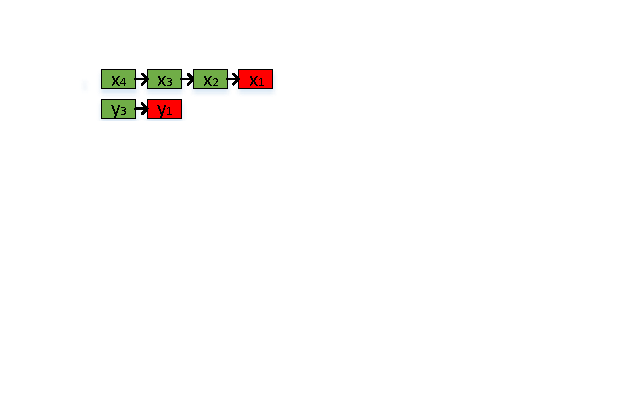
\includegraphics[scale=1.5] {figure/version1} \label{fig:versions_a}}
    \captionsetup[subfigure]{margin={0cm,0cm}
  }
  \subfloat[\small ${H_b = H_a c_2r_5[y_3]w_6[x_4]}$]
  {
    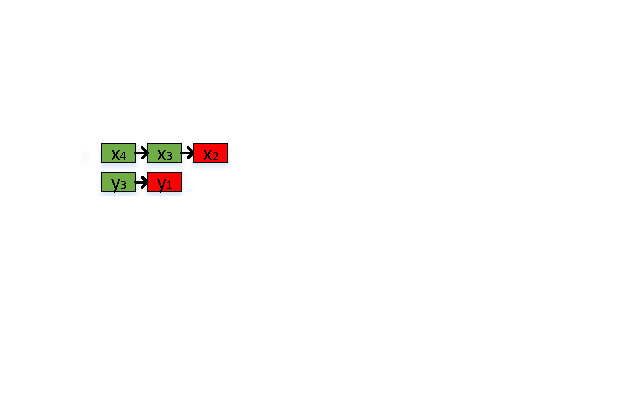
\includegraphics[scale=1.5]{figure/version2} \label{fig:versions_b}
  }
    \captionsetup[subfigure]{margin={0cm,0cm}
  }
  \subfloat[\small ${H_c = H_b a_3a_5}$]
  {
    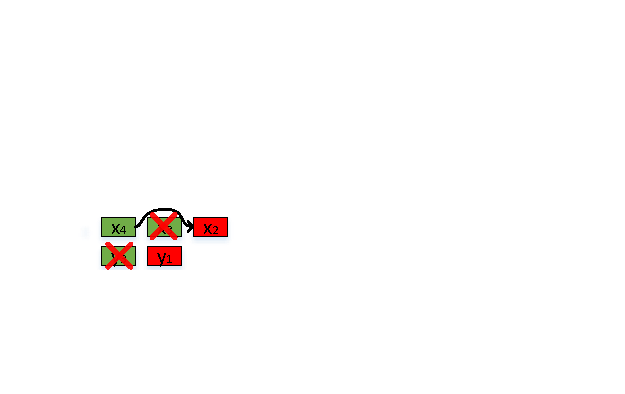
\includegraphics[scale=1.5] {figure/version3} \label{fig:versions_c}}
    \captionsetup[subfigure]{margin={0cm,0cm}}
    \subfloat[\small ${H_d = H_c c_4r_6[y_1]c_6}$]
      { 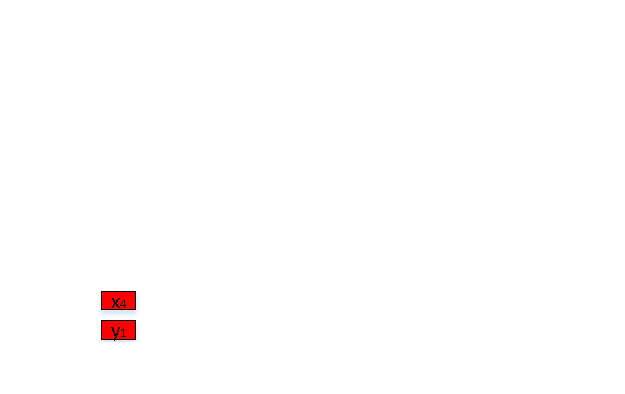
\includegraphics[scale=1.5]{figure/version4} \label{fig:versions_d}
  }
  \caption{speculative(green) and committed(red) versions,
  ${x_i}$ express this version is from transaction transaction ${T_i}$'s write.
So, $w_j[x_i]$ express transaction ${T_j}$ overwrite ${T_i}$'s write. 
}
\label{fig:versions_example}
\end{figure}

\subsection {Lock Violation Occasion}


In a distributed transaction, $TM$ assigns work to $RM$. Once the work is done, $TM$ applies 2PC to end the transaction.
In 2PC, both $TM$ and $RM$ need to synchronize with their replicas, to make sure that node failures will not corrupt the data.
Synchronization usually takes a long time, especially when the replicas are located remotely.
DLV aims to prevent data synchronization from coinciding with the lock holding time.


In \emph{late lock violation}, a transaction allows its lock to be violated only after all $RM$s confirm that they can commit.
Therefore, it requires an additional message round trip between the $TM$ and the $RM$s before the commit starts.
In \emph{early lock violation}, each $RM$ can autonomously decide to when to permit lock violation. 
It saves a message round trip, but faces a higher chance of cascade abort.
We implement 4 types of DLV strategies which are different on viollation time.
The lock violation time in \emph{DLV0}, \emph{DLV1}, \emph{DLV1}, \emph{DLV2} is following:

\emph{DLV0}: once a transaction has finished an access operation, the lock which protects this operation can be violated;

\emph{DLV1}: when a transaction in an ${RM}$ has decides its prepare status, the locks on this shard hold by this transaction can be violated;

\emph{DLV1x}: a transaction ensures all the ${RM}$ related has decides their prepare, all the transactions's lock can be violated;

\emph{DLV2}: a transaction enter 2 phase of 2PC, all of the transactions's lock can be violated.

\emph{DLV0} and \emph{DLV1} is early lock violation, and \emph{DLV1x} and \emph{DLV2} is late lock violation.
DLVx implementation \emph{late lock violation} by adding a message round trip to prevent deterministic abort when use lock violation.
This additional message flow shows in Fig~\ref{fig:two_layers_architecture}, the message is show as dotted arrow lines.
Before an ${RM}$ decides to replicate its prepare log, it also sends a \emph{Ready} message to ${TM}$ and tells ${TM}$ it will prepare this transaction.
\emph{Ready} message shows that the ${RM}$ will prepare commit or prepare abort.
When the \emph{TM} collect all \emph{RM}s \emph{Ready} message, it sends \emph{Violate} messages to tells every \emph{RMs} make their locks are violative.
An interactive-transaction can combine these messages with the last operations and prepare requests in passing, as Fig~\ref{fig:transaction_interactive} shows.
So, the interactive transaction needs no dynamic decides the lock violation time.
Interactive transactions use DLV would only work as \emph{late violation}.
We mainly focus on discuss one-shot transaction model here.
For a one-shot transaction, this message flow also takes less time than the overall message flow of 2PC because of no log replication time dealy.
Especially when all the ${RMs}$ and the ${TM}$ are located in LAN, there is no WAN message RTT.


\subsection {Deadlock Prevention and Dependency Tracing}

DLV adopts the \emph{wait-die} protocol to prevent deadlocks and dependency cycles.
A transaction is assigned a unique timestamp when it starts.
Conflicting transactions can then be ordered by their timestamps.
Once a transaction attempts to access a data item locked by a transaction with a larger timestamp, the transaction is aborted.
As mentioned earlier, this is a simple and effective approach in a distributed environment.
The conflict transaction operations are queued base their transaction id's order.
In early lock violation mode, 
DLV would consolidating all the wait in the final wait.
Ealy lock violation also obeys \emph{wait-die} rule.
A transaction can only violate a lock with greater transaction id,
which is the same as wait rule.
By this approach, transaction dependencies graph can not create a circle.
It can reduce possible false positive abort when exploit early lock violation.

DLV applies the register-and-report method~\cite{HeckatonMVCC:journals/pvldb/LarsonBDFPZ11} to trace commit dependencies among transactions.
Each transaction maintains an in-dependency count (${in}$ attribute of Context in Algorithm \ref{alg:struct}), which records how many transactions it depends on.
At the same time, each transaction also maintains an out-dependency transaction set (${out}$ attribute of Context in Algorithm \ref{alg:struct}), which records all the transactions depending on it.
When a transaction ${T}$ reads from ${S}$,
DLV registers the commit dependency by adding ${T}$ to the ${out}$ set of ${S}$ and incrementing ${in}$ of ${T}$ by one.
%These steps are described by line 4 - 7 in function READ in Algorithm \ref{alg:execution_phase}.
A transaction cannot start committing if it's ${in}$ value is greater than 0, which means some of its in-dependency transaction has not committed yet.
When a transaction aborts, it may cause its out-dependency transactions abort cascadely. 
For this purpose, it notifies all its out-dependency transactions to abort too, by setting their ${in}$ values to a negative value, for example ${-\infty}$.
This means that the transaction must abort.
%Algorithm~\ref{alg:prepare_phase} shows how to prepare a transaction.
When a transaction commits, this transaction will traverse its ${out}$ set and decrease its out-dependency transactions' ${in}$ values by one.
This dependency information can be maintained in main memory.
If there is node failure, this information can be dropped safely. 

%, this is shown in line 6 - 11 of Algorithm \ref{alg:commit_phase} function. 
%Line 2 of function CASCADE in Algorithm \ref{alg:commit_phase} shows the assign ${in\_dn}$ by a negative value when cascade abort.

\subsection{Pseudocode Description}

\begin{algorithm}
  \caption{Transaction Context and Lock Structure Definination}
  \label{alg:struct}
  \begin{algorithmic}[1]
    \label{struct:context}
    \State \textbf{struct} Context $\{$
    \State \hskip2em \emph{xid}; \Comment{transaction id}
    \State \hskip2em \emph{in}; \Comment{in dependency transaction count}
    \State \hskip2em \emph{out}; \Comment{out dependency transaction set}
    \State \hskip2em \emph{locks}; \Comment{lock acquired}
    \State \hskip2em \emph{write\_set}; \Comment{write row set}
    \State \hskip2em \emph{violate};  \Comment{EARLY or LATE}
    \State  $\};$
  \end{algorithmic}

  \begin{algorithmic}[1]
    \State \textbf{struct} Lock $\{$
    \State \hskip2em \emph{xid};\Comment{transaction id}
    \State \hskip2em \emph{key};\Comment{locked key}
    \State \hskip2em \emph{mode};\Comment{lock mode, READ or WRITE}
    \State \hskip2em \emph{violate};\Comment{EARLY, LATE or NONE}
    \State  $\};$
  \end{algorithmic}
\end{algorithm}

Algorithm~\ref{alg:struct} describes the transaction context on ${RM}$ and the lock structure.
The meanings of the elements are shown in the comments.
Both these structures has a violate attribute to indicate which lock violation strategy the transaction used.
The \emph{violate} value of Context are initialized when transaction context is created.
It would be assigned by EARLY if DLV0 or DLV1 setting, and LATE if DLV1x or DLV2 setting.
Lock structure has \emph{violate} attribute which is initilized as NONE to show it cannot be violated.
Depends on lock violation strategy, it would becomes EARLY or LATE to express the lock can be violated early or late.

In Algorithm~\ref{alg:lock},  Function Lock decreases the procedure of transaction locking.
It has 4 input arguments: transaction context ${T}$, the key to lock ${K}$, lock mode ${M}$ and violation type ${V}$.
First the Lock function check if there's a conflict lock in the lock table.
It also test weather it can be violated by the current transaction.
Transaction ${T}$ can only wait a lock who hold by another transaciton has a greater transaction xid\footnote{we suppose there is no lock upgrade, so there are no conflict locks hold by one transaction}.
Otherwise, transacion ${T}$ would fail to acquire this lock and abort later.
Once any locks are violated, 
${T}$ would register its dependency if it is necessary. 
Finally, Lock return the newly created lock.


Algorithm~\ref{alg:lock_violation} inclues test violable function and enable violation function.
Function Violable return weather a transaction ${T}$ can violate lock ${L}$ on ${K}$ in ${M}$ mode.
EnableTxV enable all the locks on a shard can be violated.
EnableLkV is used to make a lock can be violated.

Algorithm~\ref{alg:execution_phase} depicts the execution phase of a transaction includes Read and Write functions.
Read and Write function would lock the read or write key.
The lock would be add to the lock set of transaction context
if the lock acquire succeed.
After the transaction access the key,
EnableLkV would be called to enable this lock violable if current database is in DLV0 setting. 

Algorithm~\ref{alg:prepare_phase} describes the prepare phase of a transaction.
When use DLV1 setting, 
transaction 
The transacion context would wait on its in dependency.
The transaction context cannot enter prepare phase if its ${in}$ value is greater than 0, which stands it has in dependency transaction.
Once ${in}$ become 0, the transaction processing can go and continue enter its prepare phase.
In some situations, there may be cascade abort.
${in}$ value less than 0 indicates ${T}$ would cascade abort. 


Algorithm~\ref{alg:commit_phase} the final phase of 2PC.
When a ${RM}$ receive \emph{Commit} message from ${TM}$, it would run Commit function.
In Commit function, transaction would test if DLV2 setting on and enable violation.
The it clean its write version , write log and release the locks.
If current transaction has out dependencies, the ${in}$ value of the dependency transaction would be decreased one.
The transaction reports the dependency transactions stop waiting  if $in$ equal 0 after the subtraction.  
Abort procedure first write the abort log, clean dirty version of this transaction and release log.
Transactions who depends on this transacion would be noticed to abort by seting their ${in}$ dependency count negative.

\begin{algorithm}[!h]
  \caption{Transaction Lock/UnLock a Key \\
  ${T}$ transaction context \\ 
  ${K}$ lock key \\
  ${L}$ the lock to be violated \\
  ${M}$ lock mode(\emph{Read} or \emph{Write}) }
  \begin{algorithmic}[1]
  \Function{Lock}{$T, K, M$}
    \State {\textbf{wait if} ${\exists}$ such ${l \in lock\_table }$,
      \newline $Conflict(K, T, l, M)$ \textbf{and}  
      \newline \textbf{not} $ Violable(K, T, l, M)$}
      \State \hskip2em \textbf{if}  {${T.xid > l.xid } $}
          \State \hskip4em  \textbf{return} nil \Comment{lock die error}
      \State \hskip2em \textbf{end if} 
    \State \textbf{end wait}

    \ForAll {such ${l \in lock\_table}$, \\ ${Violable(K, T, l, M) }$}
        \State {${s \gets}$  transaction context retrieved by ${l.xid}$}
        \If {${T.violate = EARLY}$ \textbf{or} $($ ${T.violate = LATE}$ 
        \newline 
        \textbf{and} 
        ${l.lmode = WRITE}$ \textbf{and} ${M = READ}$ $)$}
        \If {${T.xid \notin s.out }$}
          \State ${s.out\_set \gets s.out \cup T.xid}$
          \State ${T.in \gets T.in + 1}$
        \EndIf
        \EndIf
    \EndFor
    \State {create lock ${l' \gets \{T.xid, K, M, None\}}$}
    \State  \textbf{return} lock ${l'}$
  \EndFunction
  \label{func:lock}
  \end{algorithmic}

  \begin{algorithmic}[1]
    \Function{UnLock}{$T, K$}
      \If {${ \exists l \in lock\_table}$,  ${l.xid = T.xid}$ \textbf{and} \\ ${l.key = K}$}
        \State {remove such $l$ from ${lock\_table}$}      
      \EndIf
    \EndFunction
    \label{func:conflict}
    \end{algorithmic}


  \begin{algorithmic}[1]
  \Function{Conflict}{$K, T, L, M$}
    \If {${T.xid \neq L.xid}$ \textbf{and} ${K = L.key}$}
      \State \textbf{return} L.lmode = WRITE \textbf{or} M = WRITE
    \Else
      \State \textbf{return} \textbf{false}
    \EndIf
  \EndFunction
  \label{func:conflict}
  \end{algorithmic}


  \label{alg:lock}
\end{algorithm}


\begin{algorithm}[!h]
  \caption{Lock Violation Test and Enable Violation \\
  ${T}$ transaction context \\ 
  ${K}$ lock key \\
  ${L}$ the lock to be violated \\
  ${M}$ lock mode \\
  ${VT}$ violation type, EARLY or LATE}
 
  \begin{algorithmic}[1]
  \Function{Violable}{$T,K, L, M$}
  \If {$CONFLICT(K, T, L, M)$ \textbf{and}\\ ${L.violate \neq NONE}$}
  \If{${L.violate=EARLY}$ \\ \textbf{and} ${T.violate=EARLY}$}
    \State \textbf{return} ${T.xid < l.xid}$
  \ElsIf{${L.violate=LATE}$}
    \State \textbf{return} \textbf{true}
  \EndIf
  \Else
  \State \textbf{return} \textbf{false}
  \EndIf
  \EndFunction
  \label{func:lock_vioation}
  \end{algorithmic}

  \begin{algorithmic}[1]
    \Function{EnableTxV}{$T, VT$}
    \ForAll {$ l \in T.locks$}
      \State${l.violate \gets VT}$
    \EndFor
    \EndFunction
    \label{func:make_tx_violable}
  \end{algorithmic}

  \begin{algorithmic}[1]
    \Function{EnableLkV}{$L, VT$}
      \State${l.violate \gets VT}$
    \EndFunction
    \label{func:make_tx_violable}
  \end{algorithmic}
  \label{alg:lock_violation}
\end{algorithm}

\begin{algorithm}[!h]

  \caption{Execution Phase of Transaction \\
  ${T}$ transaction context \\ 
  ${K}$ read/write key \\
  ${V}$ value write}

  \begin{algorithmic}[1]
  \Function{Read}{$T, K$}
    \State ${l \gets Lock(T, K, READ)}$
    \If{${l}$ is ${nil}$}
      \State \textbf{return} lock failed \Comment{${T}$ will abort later}
    \Else
      \State ${T.locks \gets T.locks \cup l}$
      \State if DLV0 setting, \textbf{call} $EnableLkV(l, EARLY)$
      \State \textbf{return} ${v}$
    \EndIf
  \EndFunction
  \label{func:read}
  \end{algorithmic}


  \begin{algorithmic}[1]
  \Function{Write}{$T, K, V$}
  \State ${l \gets Lock(T, K, WRITE)}$
  \If{${l}$ is ${nil}$}
    \State \textbf{return} lock failed
    \Comment{${T}$ will abort later}
  \Else
    \State ${T.locks \gets T.locks \cup l}$
    \State assign ${K}$'s newest version by value ${V}$
    \State add tuple to ${T.write\_set}$
    \State if DLV0 setting, \textbf{call} $EnableLkV(l, EARLY)$
    \State \textbf{return} write success
  \EndIf
  \label{func:write}
  \EndFunction
  \end{algorithmic}
  \label{alg:execution_phase}
\end{algorithm}

\begin{algorithm}[!h]
  \caption{Prepare Phase of Transaction ${T}$}
  \begin{algorithmic}[1]
  \Function{Prepare}{$T$}
      \State if DLV1 setting, \textbf{call} ${EnableTxV(T, EARLY)}$
      \State if DLV1x setting, issue $TM$ a \emph{\{Ready\}} message.


    \State \textbf{wait} \textbf{if} ${T.in > 0}$
    \If {${T.in < 0}$}
      \State write prepare abort log
      \State response \emph{TM} message \emph{\{Prepare Abort\}} \Comment{cascade}
    \ElsIf {$T.in = 0$}
      \State write prepare commit log
      \State response \emph{TM} message \emph{\{Prepare Commit\}} 
    \EndIf
  \EndFunction
  \end{algorithmic}
  \label{alg:prepare_phase}
\end{algorithm}

\begin{algorithm}[!h]
  \caption{Commit/Abort Phase of Transaction ${T}$}
  \begin{algorithmic}[1]
  \Function{Commit}{$T$}
    \State if CLV2 setting, \textbf{call} ${EnableTV(T)}$ 
    \State write commit log
    \ForAll {${r \in T.write\_set}$}
      \State make the version written by ${T}$ becomes commit version of tuple ${t}$ 
    \EndFor
    \ForAll {$ l \in T.locks$}
      \State UNLOCK(${l}$)
    \EndFor
    \For {${t \in T.out}$}
      \State ${t.in \gets t.in - 1}$ \Comment{keep exactly once}
      \If {${t.in = 0}$}
        \State report ${t.in = 0}$ \Comment{stop waiting on ${t}$}
      \EndIf
    \EndFor
    \State response \emph{TM} message \emph{\{Commit ACK\}}
    \label{func:commit}
  \EndFunction
  \end{algorithmic}
  \begin{algorithmic}[1]
  \Function{ABORT}{$T$}
  \State write abort log
  \ForAll {${r \in T.write\_set}$}
    \State remove the version written by ${T}$ in ${r}$
\EndFor

    \ForAll {$ l \in T.locks$}
      \State UNLOCK(${l}$)
    \EndFor
    \For {${t \in T.out}$}
      \State ${t.in \gets -\infty }$
      \State report ${t.in < 0}$ \Comment{stop waiting on ${t}$}
    \EndFor
    \State response \emph{TM} message \emph{\{Abort ACK\}}
    \label{func:abort}
  \EndFunction
  \end{algorithmic}

  \label{alg:commit_phase}
\end{algorithm}

\section{Experiments and Evaluations}
\label{sec:experiments}
We develop a replicated distributed DBMS demo and evaluate implement 4 types of DLV, as we disscuss previously.
As a comparison with DLV, we also implement S2PL wait die(S2PL) scheme.


\subsection{Experiments Setting}
Our experiments performed on a cluster of 13 Aliyun ecs.g6.large server.
In which one node is used to issue transaction requests.
Each server has 2 virtual CPU with 2.5GHz clock speed, 8GB RAM, runs Ubuntu 18.04.
The data is partitioned by 4 shards, each shard has 3 replicas which is replicated across 3 AZs, which is located at Heyuan, Hangzhou and Zhangjiakou.
Every AZ has a full data copy of each shard.
The internal network bandwidth of each AZ is 1Gbps.
We choose a modifies version TPCC and YCSB workload.
All the transactions are distributed transactions.
The TPCC data is sharded by the warehouse id.
The Item table is replicated to all shards.
Each transaction will retry after 3 seconds if it aborts for violation serializability.
The evaluation both tested on both scattered (leader) mode and gathered (leader) mode.
In gathered mode, all of the replica leaders are located in the same AZes.
In scattered mode, the replica leaders are not located in the same AZes.

\subsection{TPCC Performance Evaluation}

TPC-C specification models a realword workload.
TPC-C models a company has many warehouses and district, customers order their products.

In our version TPC-C benchmark,
We exclude think time of TPCC and only NewOrder procedure is used.
The data is partitioned on shards by warehouse id.
The item table is replicated by all the shard.
We also extends TPC-C workload make all the transactions are distributed transaction by enforce every order has item from different warehouse located different node.

First we simulate log cost on different an LAN environment by adding log write latency.
Fig \ref{fig:new_order_add_log_cost} shows the throughput and abort rate of TPCC NewOrder procedure on 4 shards. 
Every shards replicated transactional log with user setting latency time.
The result shows that late violation can perform better when there is a large log replicaiton latency.

\begin{figure}[htbp]
  \centering
  \captionsetup[subfigure]{margin={0cm,0cm}}
  \subfloat[NewOrder TPM]
      { 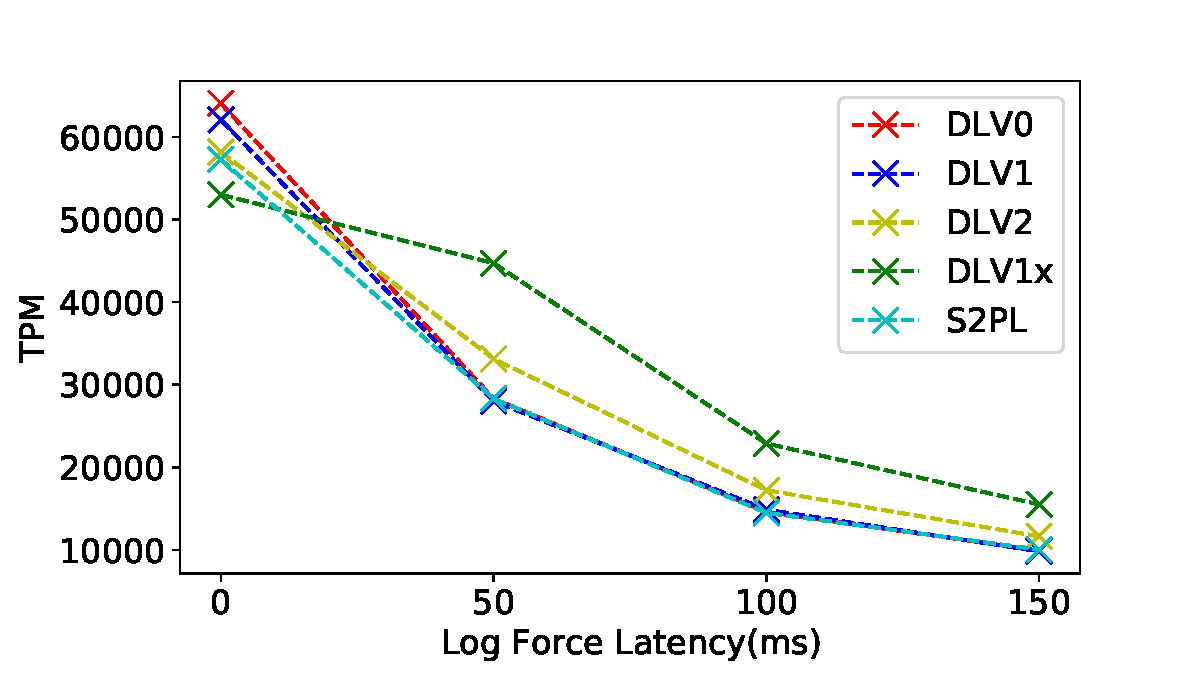
\includegraphics[scale=0.25] {figure/plot_tpcc_neworder_add_LogForceT_LogForceT_TPM_gather} \label{fig:new_order_add_log_cost:tpm}}
  \captionsetup[subfigure]{margin={0cm,0cm}}
  \subfloat[NewOrder abort]
      { 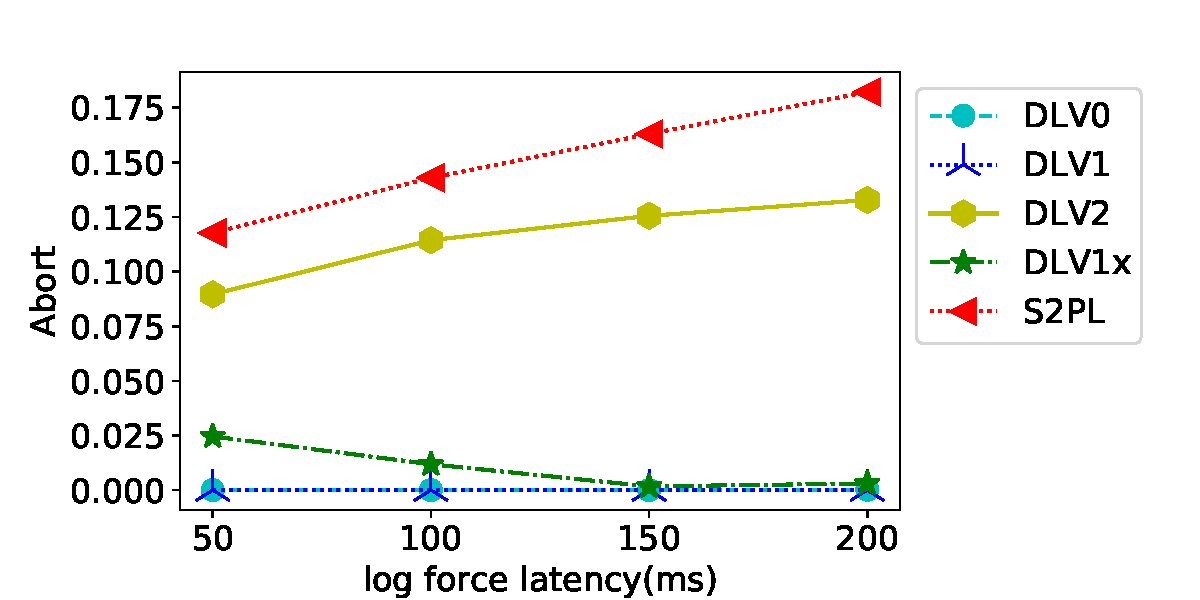
\includegraphics[scale=0.25]{figure/plot_tpcc_neworder_add_LogForceT_LogForceT_Abort_gather} \label{fig:new_order_add_log_cost:abort}}
  \captionsetup[subfigure]{margin={0cm,0cm}}
\caption{throughput and abort rate of
different terminal different log write costs}
\label{fig:new_order_add_log_cost}
\end{figure}


In the following experiments,
we all run test on a real replication environment.

Fig \ref{fig:plot_tpcc_neworder_add_Warehouse_Warehouse_gather} is the performance comparation of different warehouse number.
DLV perform better when warehouse number is small.
The less warehouse number the data divided, the more contention the transaction would incur.
DLV only optimize contention wrokload.
DLV1x perform better among other approach various on may warehouse number.


Fig \ref{fig:new_order_add_terminal_gathered} shows the NewOrder performance of when adding terminal numbers of each node in the gathered mode.
In gathered mode, message between replica leaders has the minimize RTT.
DLV1x can benefit from less RTT cost.
DLV1x scale well when adding terminal number of each shard.
Fig \ref{fig:new_order_add_terminal_scattered} shows that even in scattered mode, leader communication has more cost.
DLV1x perform better than other DLV strategies.


\begin{figure}[htbp]
  \centering
  \captionsetup[subfigure]{margin={0cm,0cm}}
  \subfloat[NewOrder TPM]
      { 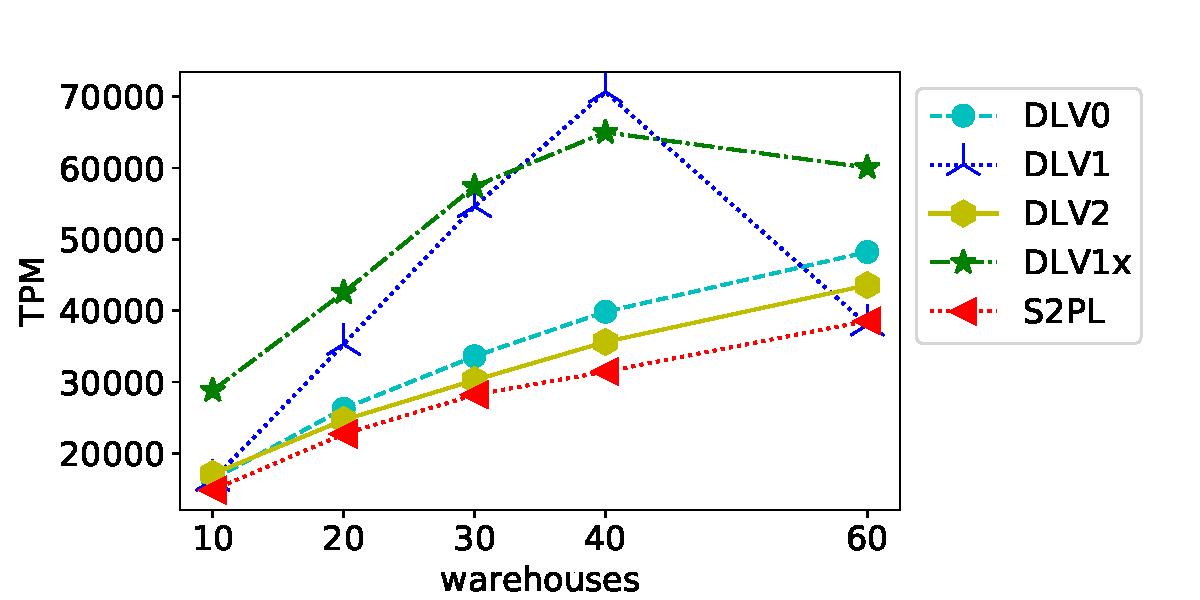
\includegraphics[scale=0.25] {figure/plot_tpcc_neworder_add_Warehouse_Warehouse_TPM_gather} \label{fig:plot_tpcc_neworder_add_Warehouse_Warehouse_gather:tpm}}
  \captionsetup[subfigure]{margin={0cm,0cm}}
  \subfloat[NewOrder abort]
      { 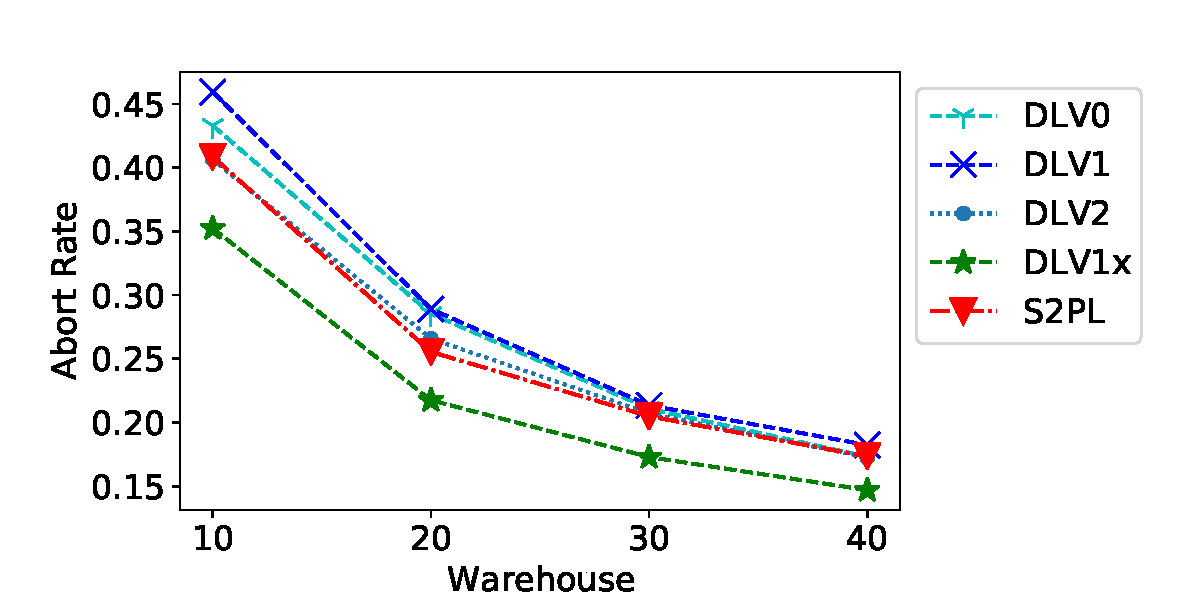
\includegraphics[scale=0.25]{figure/plot_tpcc_neworder_add_Warehouse_Warehouse_Abort_gather} \label{fig:plot_tpcc_neworder_add_Warehouse_Warehouse_gather:abort}}

\caption{throughput and abort rate of
different warehouse numbers}
\label{fig:plot_tpcc_neworder_add_Warehouse_Warehouse_gather}
\end{figure}


\begin{figure}[htbp]
  \centering
  \captionsetup[subfigure]{margin={0cm,0cm}}
  \subfloat[NewOrder throughput]
      { 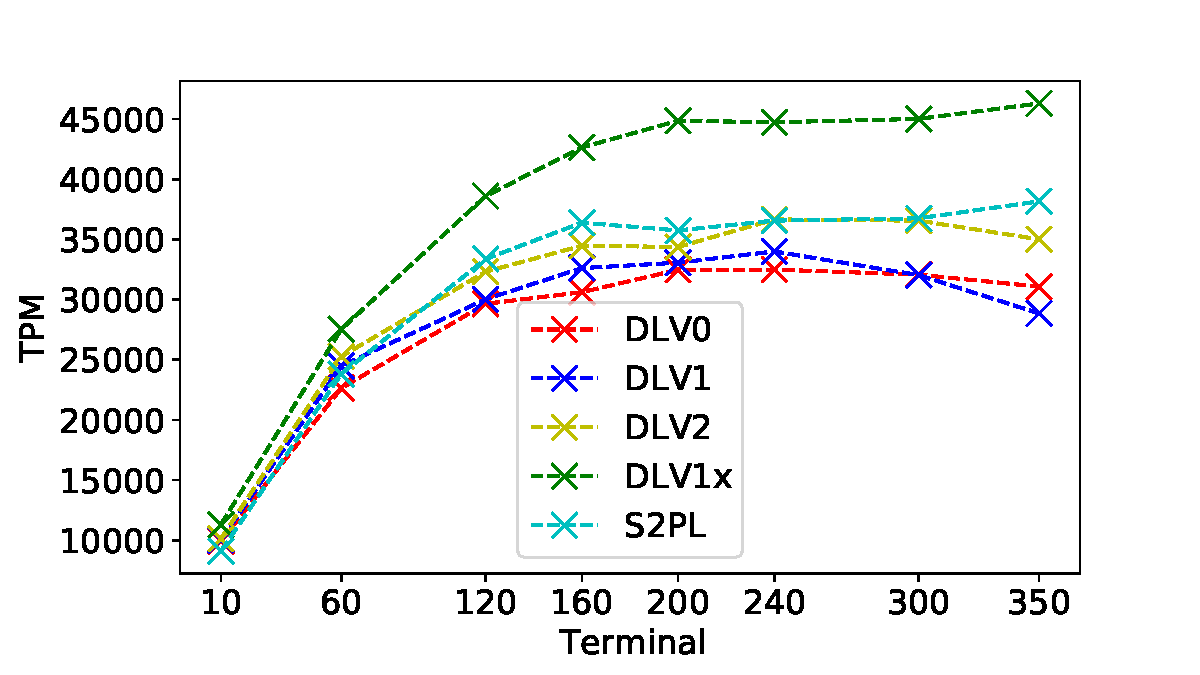
\includegraphics[scale=0.25] {figure/plot_tpcc_neworder_add_Terminal_Terminal_TPM_gather} \label{fig:new_order_add_terminal_gathered:tpm}}
  \captionsetup[subfigure]{margin={0cm,0cm}}
  \subfloat[NewOrder abort rate]
      { 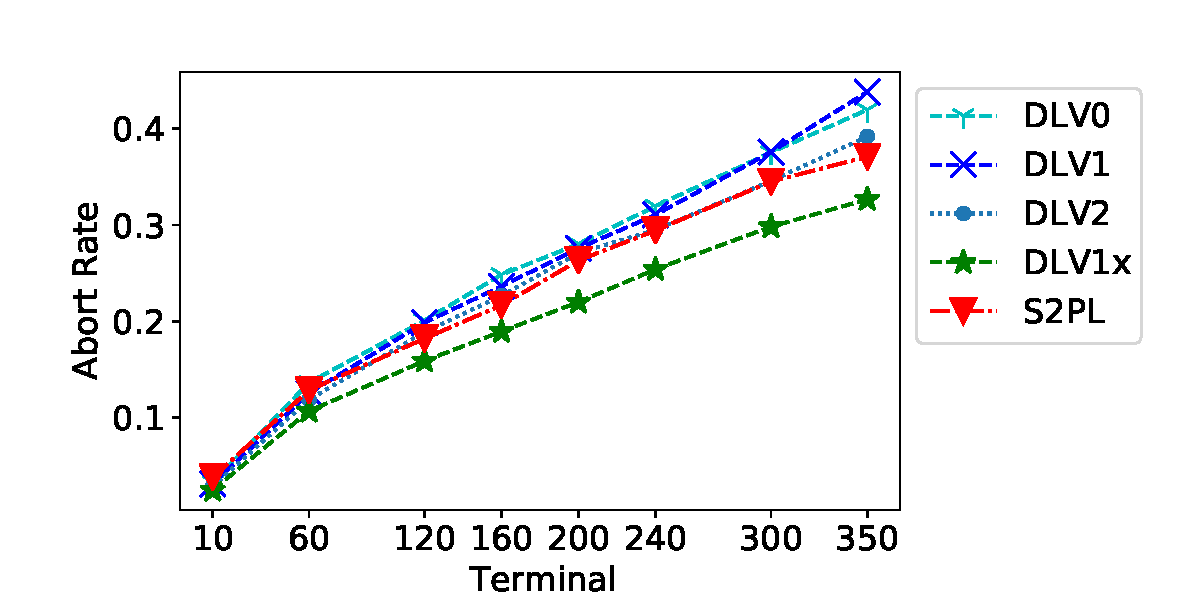
\includegraphics[scale=0.25]{figure/plot_tpcc_neworder_add_Terminal_Terminal_Abort_gather} \label{fig:new_order_add_terminal_gathered:abort}}

\caption{throughput and abort rate when adding terminal number of each shard, in gathered mode}
\label{fig:new_order_add_terminal_gathered}
\end{figure}


\begin{figure}[htbp]
  \centering
  \captionsetup[subfigure]{margin={0cm,0cm}}
  \subfloat[NewOrder throughput]
      { 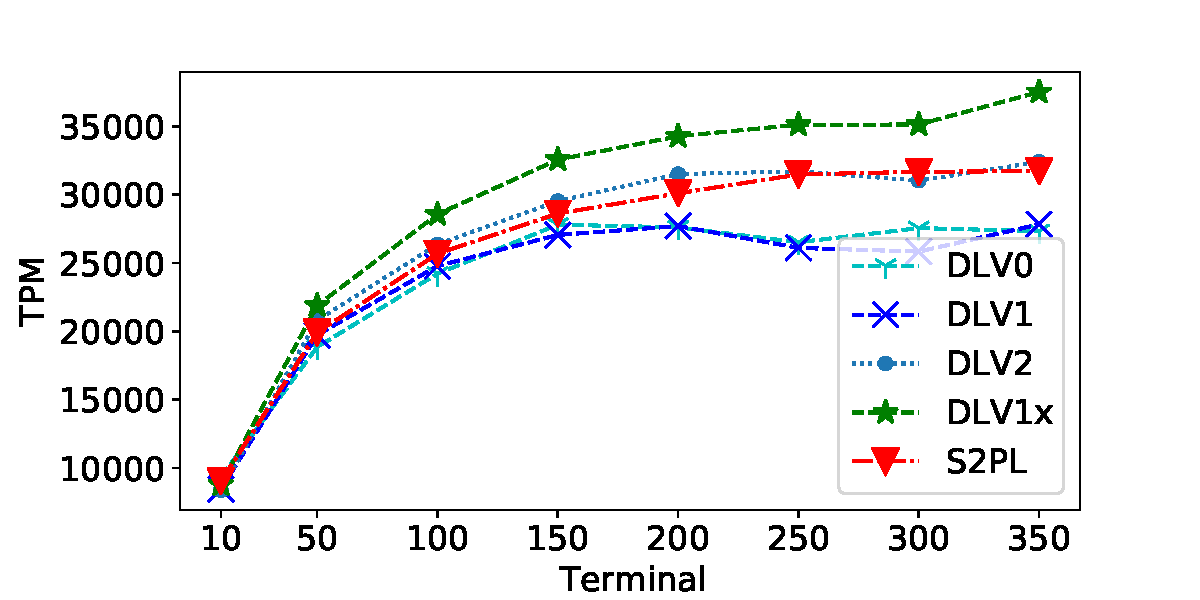
\includegraphics[scale=0.25] {figure/plot_tpcc_neworder_add_Terminal_Terminal_TPM_scatter} \label{fig:new_order_add_terminal_scattered:tpm}}
  \captionsetup[subfigure]{margin={0cm,0cm}}
  \subfloat[NewOrder abort rate]
      { 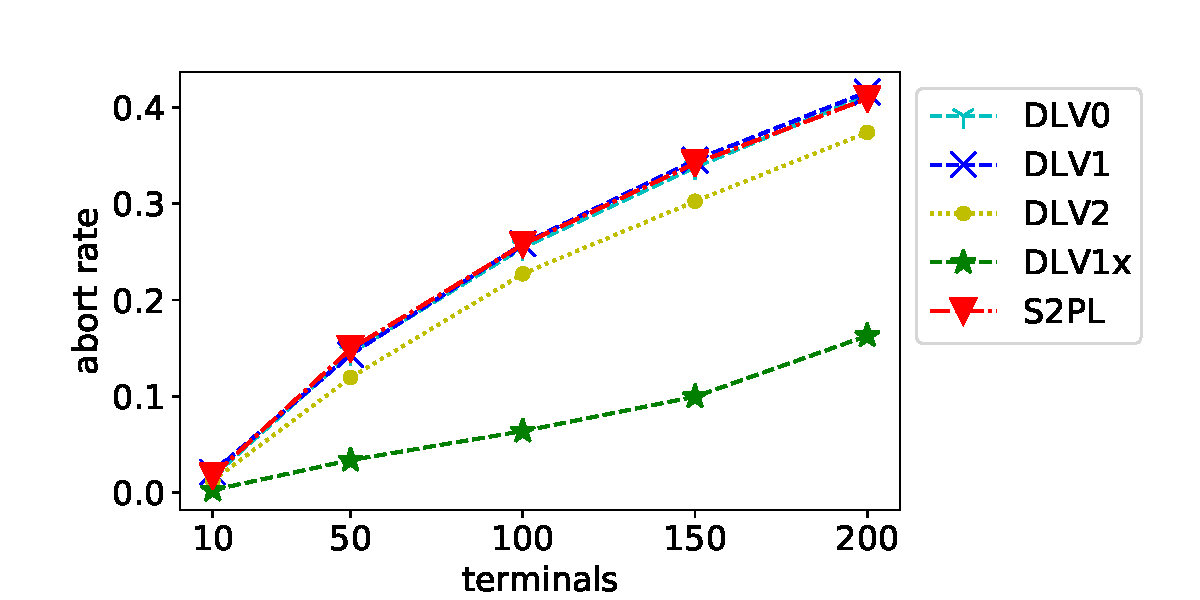
\includegraphics[scale=0.25]{figure/plot_tpcc_neworder_add_Terminal_Terminal_Abort_scatter} \label{fig:new_order_add_terminal_scattered:abort}}

\caption{throughput and abort rate when adding terminal number of each shard, in scattered mode}
\label{fig:new_order_add_terminal_scattered}
\end{figure}


\subsection{YCSB Performance Evaluation}

In YCSB workload, 

We evaluate different data skew.


\begin{figure}[htbp]
  \centering
  \captionsetup[subfigure]{margin={0cm,0cm}}
  \subfloat[YCSB work throughput]
      { 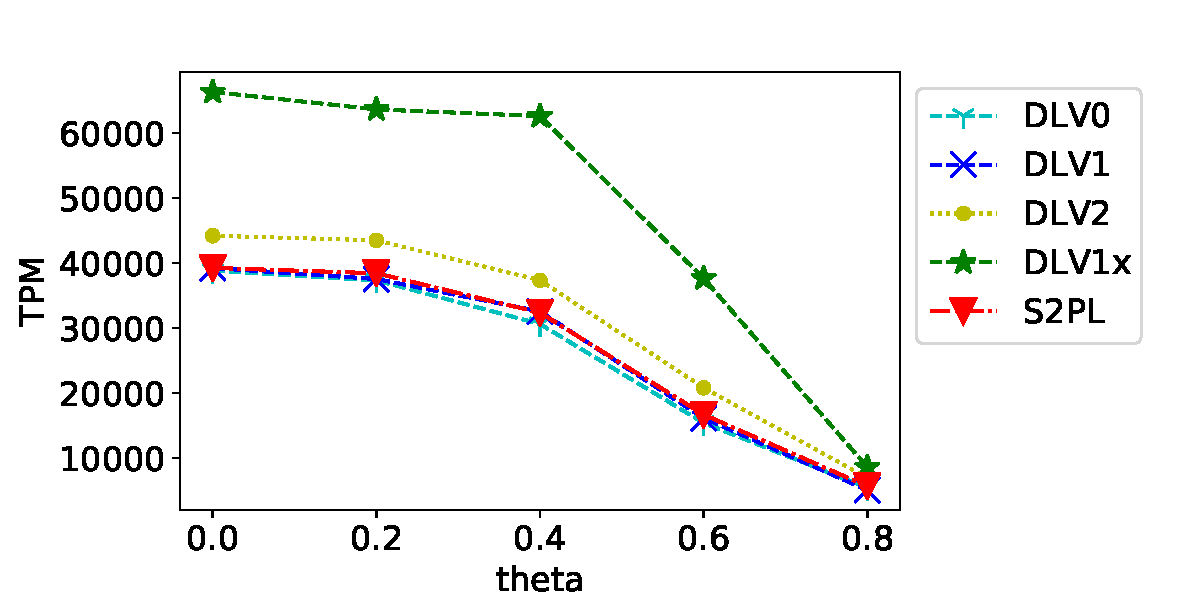
\includegraphics[scale=0.25] {figure/plot_ycsb_add_Theta_Theta_TPM_gather} \label{fig:plot_ycsb_add_Theta_Theta_TPM_gather:tpm}}
  \captionsetup[subfigure]{margin={0cm,0cm}}
  \subfloat[YCSB workload abort rate]
      { 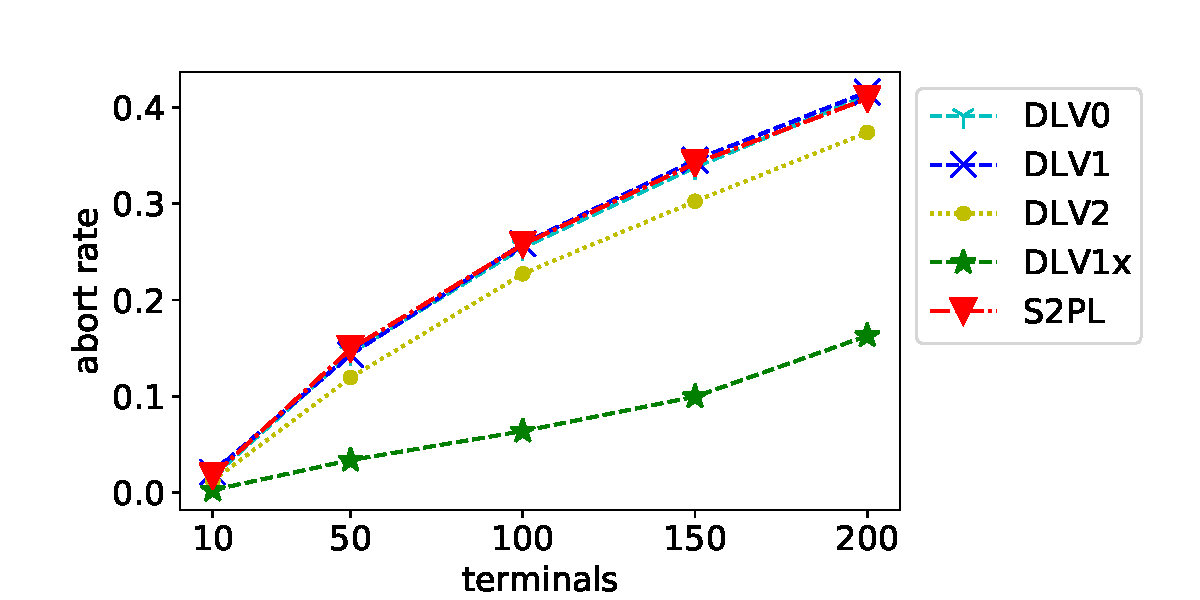
\includegraphics[scale=0.25]{figure/plot_tpcc_neworder_add_Terminal_Terminal_Abort_scatter} \label{fig:plot_ycsb_add_Theta_Theta_TPM_gather:abort}}

\caption{throughput and abort rate when adding terminal number of each shard, in scattered mode}
\label{fig:plot_ycsb_add_Theta_Theta_TPM_gather}
\end{figure}


\section{Conclution}
\label{sec:conclution}
We extend $CLV$ to distributed transaction and evaluate its performance on a geo-replicated environment.
Our distributed version ${CLV}$, i.e. DLV, can dynamically decide to violate lock at the most suitable time.
DLV merge many discrete waits at transaction running time into one final wait when commit.
According to our evaluation, DLV can improve performance of contention workload for shortening critical path.
DLV can adapt to different workloads.
It minimize unnecessary dependency tracing cost and cascade abort penalty against previous work.






\bibliographystyle{reference/IEEEtran}
\bibliography{reference/IEEEexample}


\end{document}

